\chapter{The Compact Muon Solenoid Experiment}

Physics from a theoretical point of view can consider particles in terms of their kinematic 
phase space, however we cannot make direct measurements of the hard scattering process. Instead,
detectors are built to indirectly measure the energy and momenta of the final state particles.
To do this, a layered system of sub detectors is used to perform particle identification. 
By relying on known interactions of standard model particles with detector materials 
strong probabilitistic statements can be made the flavor of particles in a given collision. 
By building a heremetic detector and integrating the various subdetectors in a given 
solid angle, one obtains a wholeistic view of the fundamental physics.
This chapter will discuss each subdetector, the particles it is used to identify, and the 
underlying physics which allows the individual measurements to be made.


The Compact Muon Solenoid (CMS) Detector is a general-purpose detector consisting of 
an all silicon tracker, a precision electromagnetic calorimeter (ECAL), a hadron calorimeter
 (HCAL), a 4 T superconducting solenoid and muon chambers. The solenoid deflects charged
 particles whose paths are traced in the tracker, making it possible to 
reconstruct the particles’ momentum. The two calorimeters reconstruct the energy 
of and identify photons, electrons and hadronic jets.
As shown in Figure \ref{fig:cms} the detector has cylindrical symmetry about the
 interaction point where the proton beams collide. By maintaining near full coverage 
of the interaction point it is possible to detect signatures such as neutrinos or other 
weakly interacting particles as missing energy. 


\begin{figure}
\begin{center}
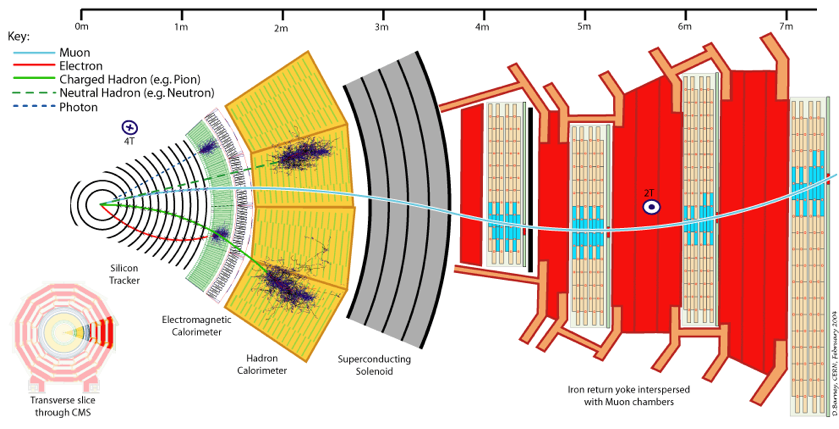
\includegraphics[width=.95\textwidth]{pics/cms_transverse}
\end{center}
\caption{ A tear-away view of the inner detectors of CMS.}
\label{fig:cms_transverse}
\end{figure}

\begin{figure}
\begin{center}
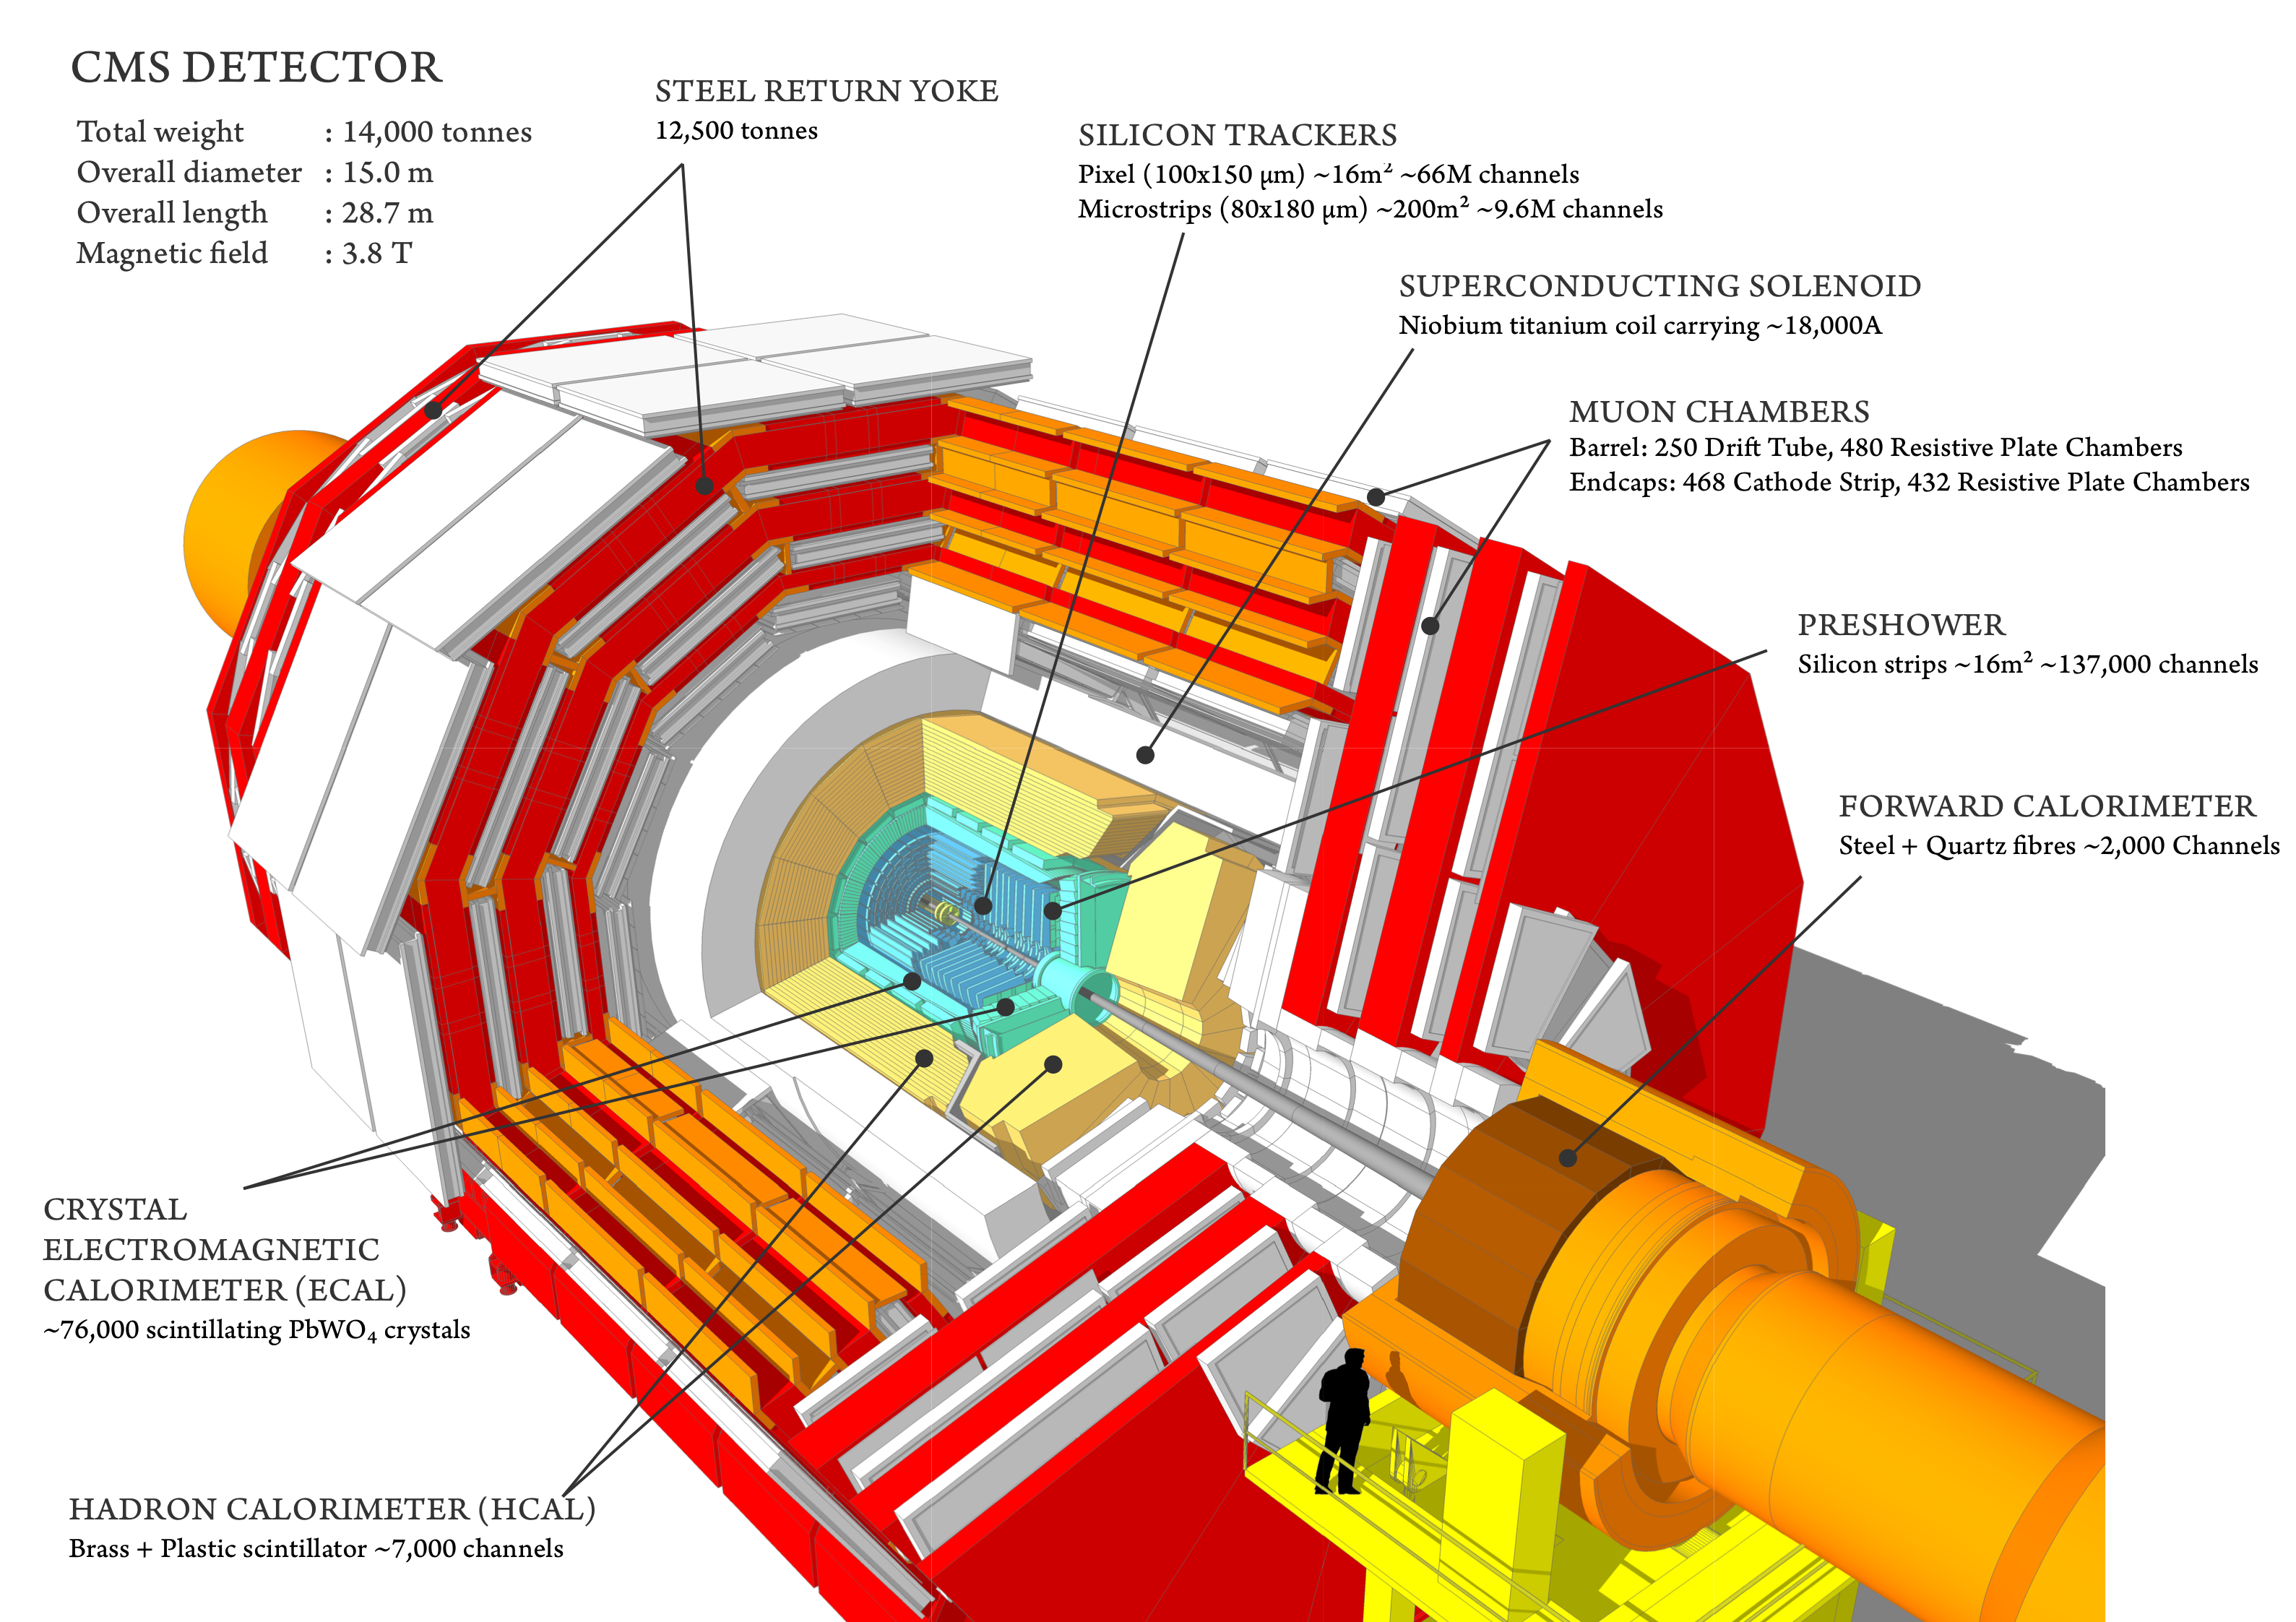
\includegraphics[width=.90\textwidth]{pics/cut_away_view}
\end{center}
\caption{Cut away view of the CMS Detector}
\label{fig:cms_onion}
\end{figure}



\section{Superconducting Solenoid}


\begin{figure}
\begin{center}
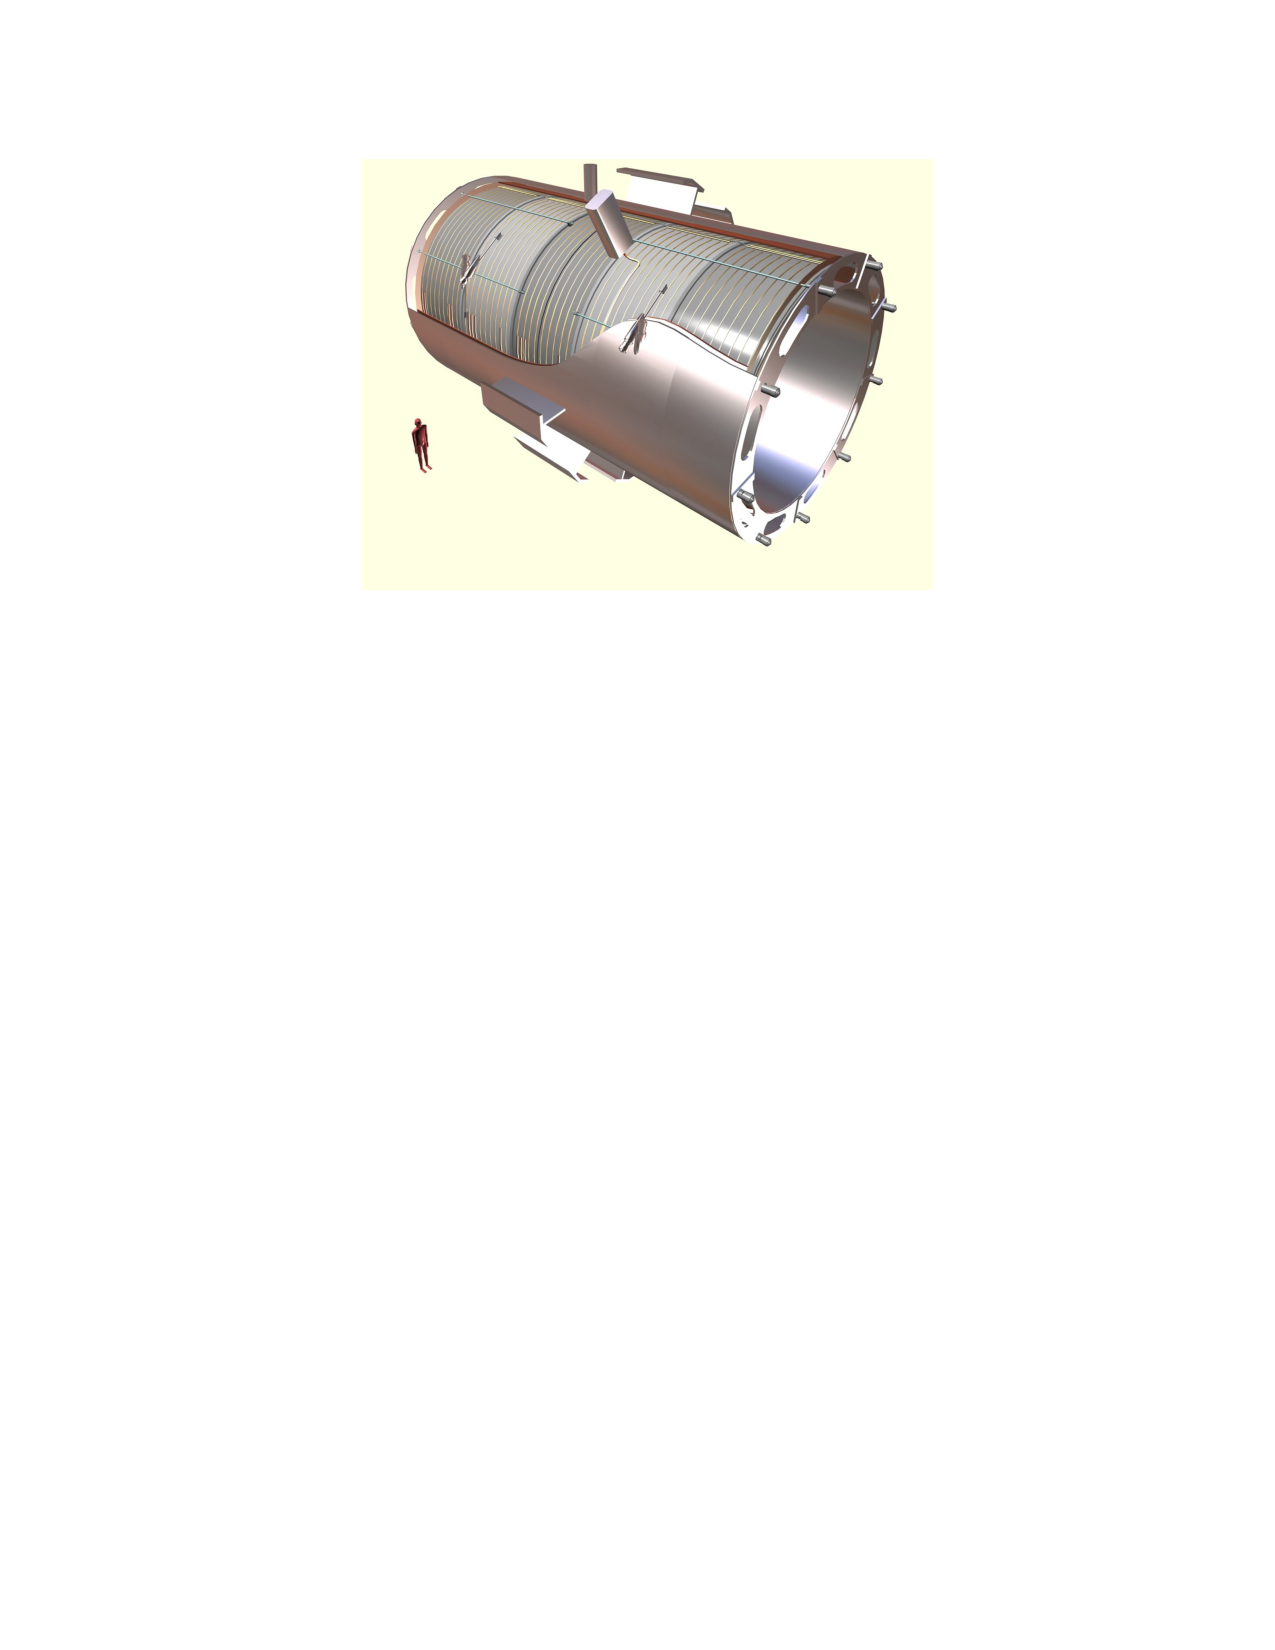
\includegraphics[width=.45\textwidth]{pics/solenoid_diagram}
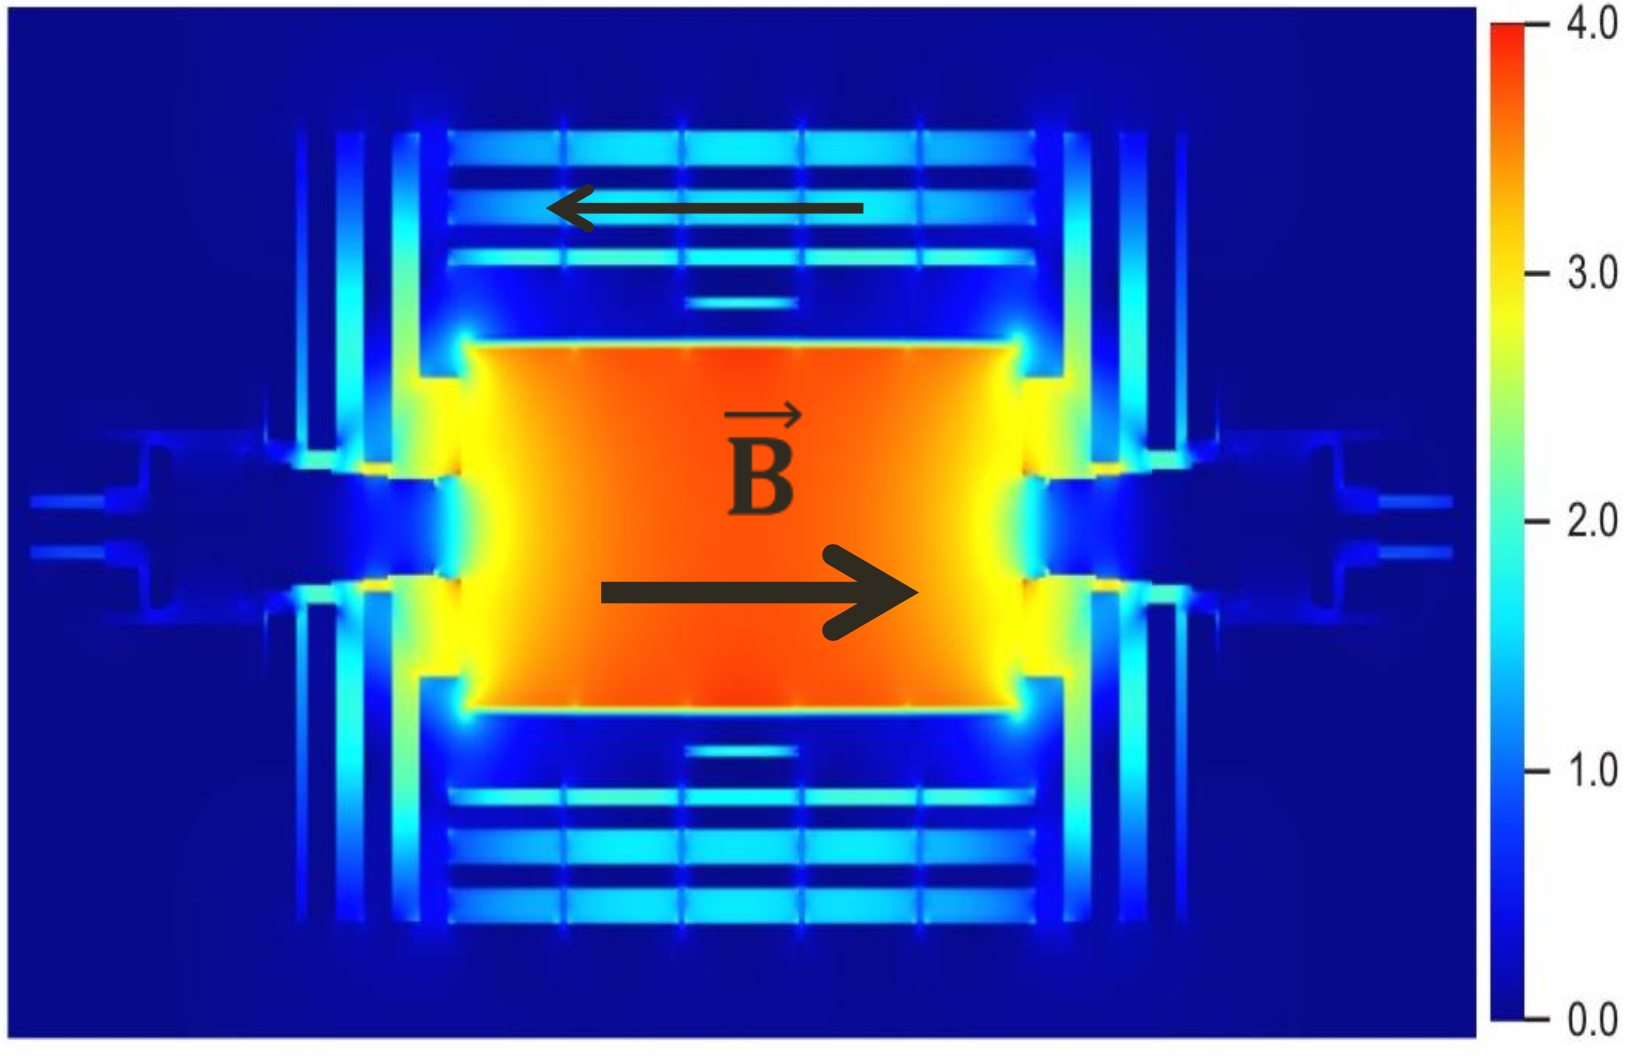
\includegraphics[width=.45\textwidth]{pics/b_field}
\end{center}
\caption{The CMS solenoid with a human for scale}
\label{fig:solenoid_bfield}
\end{figure}

It is worth beginning this discussion with the central feature the rest of the detector is built, the 
design 4 T  superconducting solenoidal magnet. For scale, a typical refridgerator magnet is on the 
order of $10^{-2}$ T and the MRI magnets can range between 0.5-3.0 T. The magnetic field is used
to measure the momentum of charged particles by bending their trajectories. As the size of the bend is
proportional to the field and inversely to the momentum of the particle, a stronger field is required 
to measure higher energy particles. 

\begin{figure}
\begin{center}
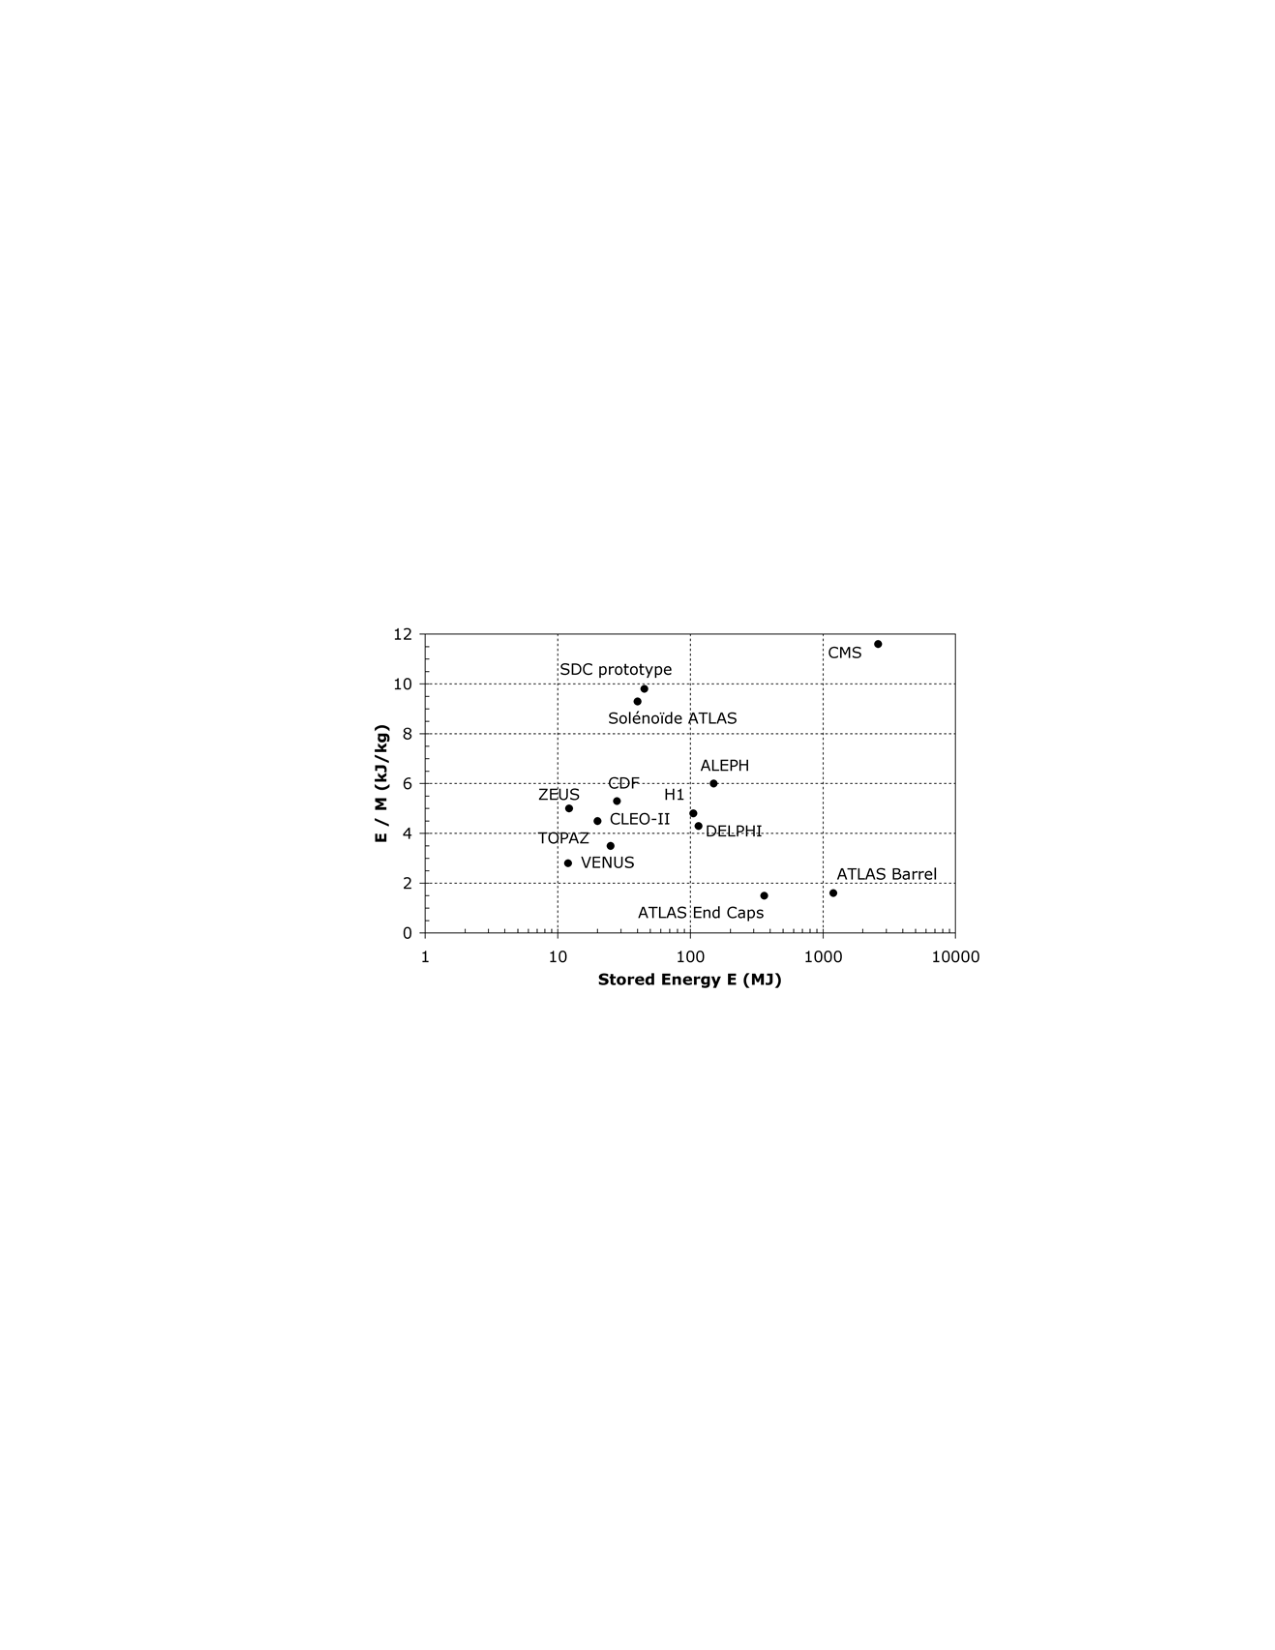
\includegraphics[width=.75\textwidth]{pics/CMS_EoverM}
\end{center}
\caption{The CMS solenoid with a human for scale}
\label{fig:eoverm}
\end{figure}

The magnet is 6 meters in diameter with 12.5 meters in length. The magnetic field is generated 2180 turns 
wound in four layers of Niobium Titanium conductors inside an alumninum cylinder carrying a
 nominal current of 20 kA.  At the design field strength the solenoid a stores magnetic field of 
2.66 GJ, the largest stored energy of any magnet ever built. The energy to mass ratio is 11.6 kJ/kG a indentifying 
feature in the historical context of detector magnets (Figure \ref{fig:eoverm}).    

\begin{figure}
\begin{center}
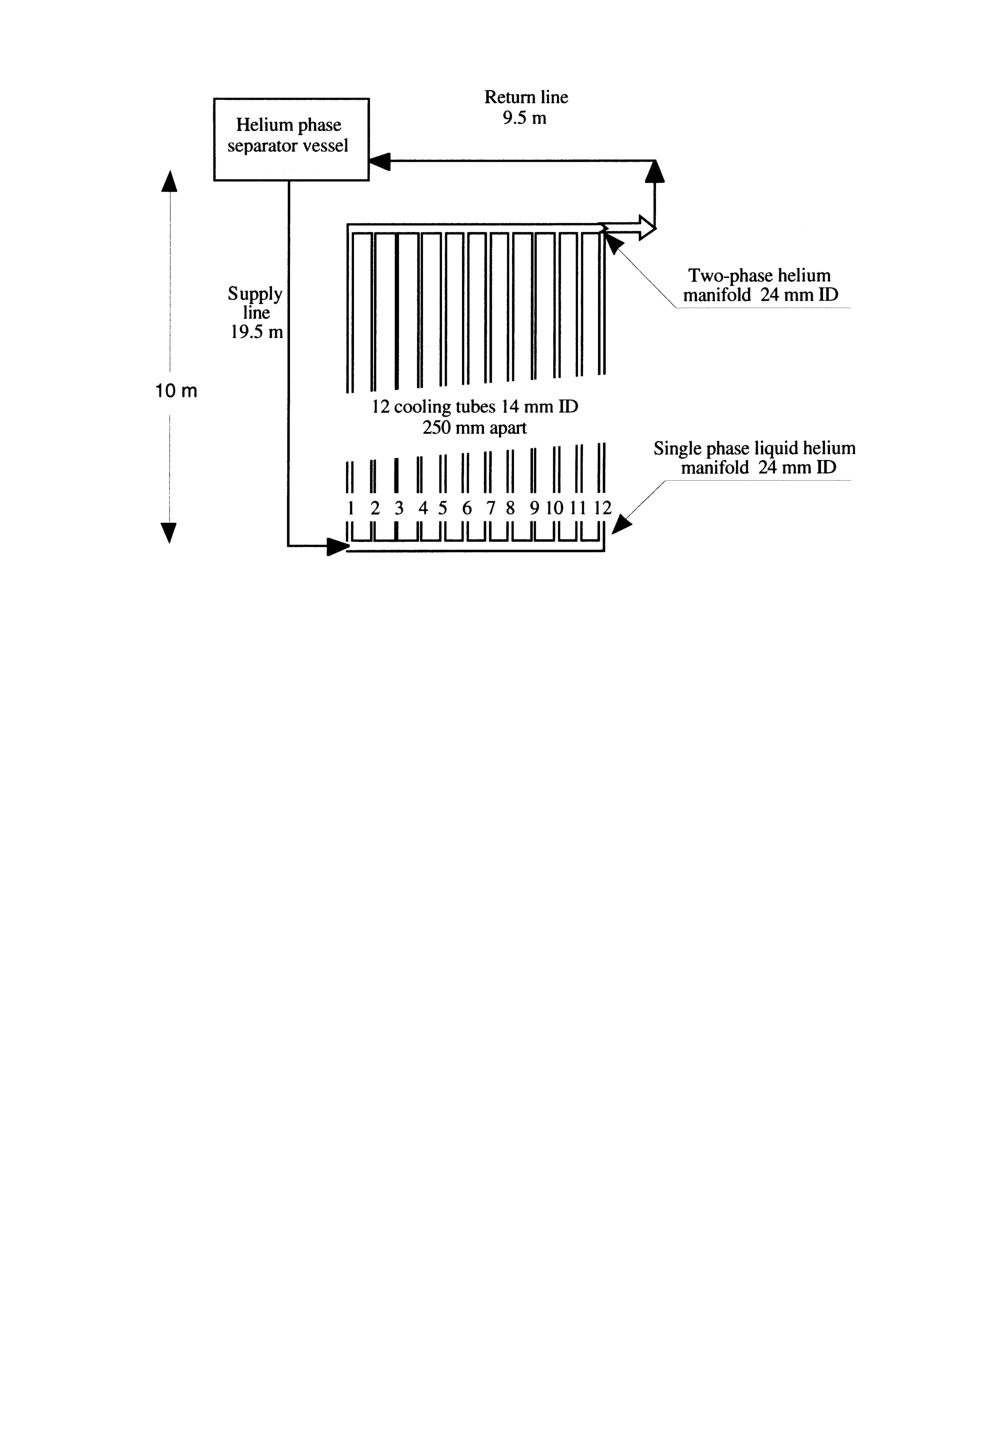
\includegraphics[width=.55\textwidth]{pics/thermosiphon}
\end{center}
\caption{A sub circuit of the CMS thermosiphon}
\label{fig:eoverm}
\end{figure}

To operate in a superconducting state, the system is cooled  4.5 K with a thermosiphon
 (cite-quench-production). A thermosiphon is an indirct cooling method utilizing passive heat exchange where
rather than pumping the liquid helium the flow is induced thermally. 

The system requires 3 days to 
reach cool the system from room to operating temperature. 

The magnet is supplemented by a iron return yoke to



\section{Electromagnetic Calorimeter (ECAL)}


\begin{figure}
\begin{center}
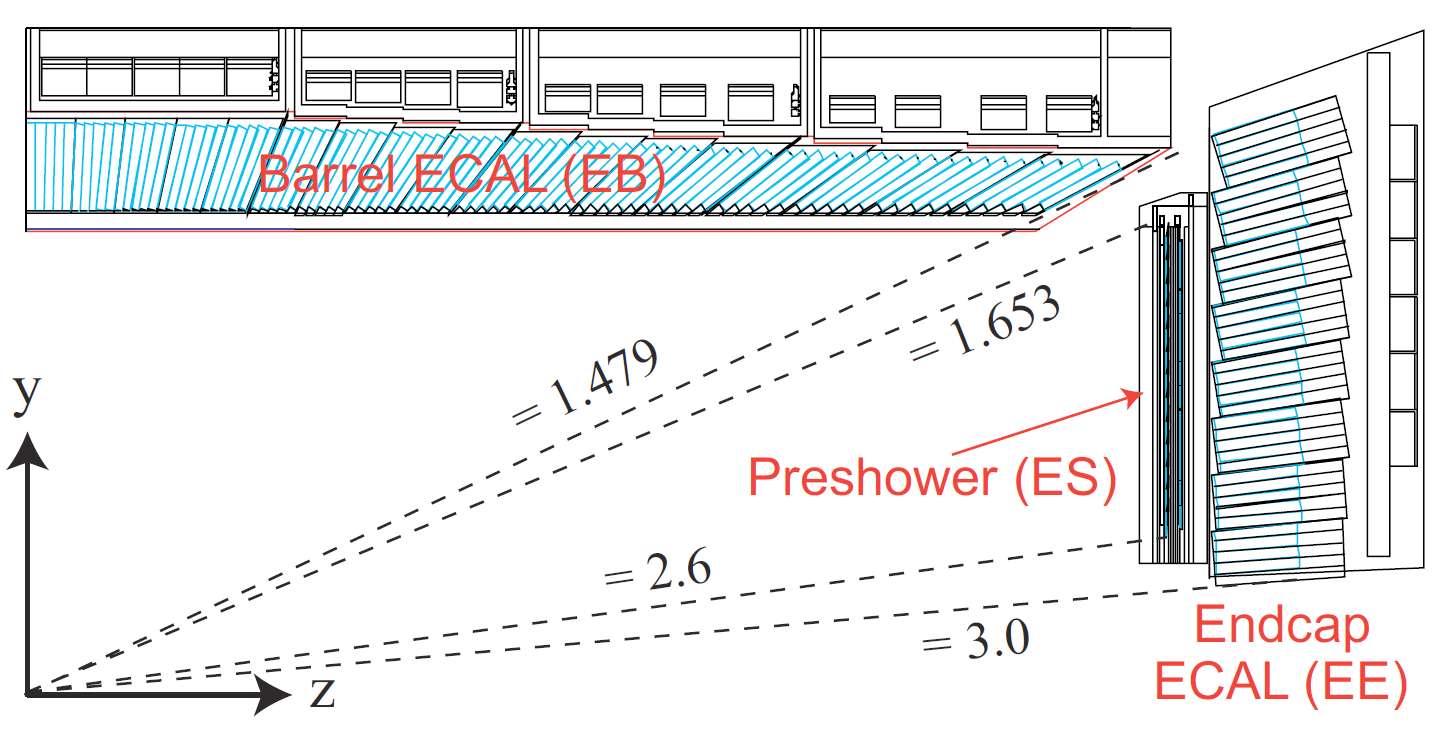
\includegraphics[width=.95\textwidth]{pics/ecal_diagram_side}
\end{center}
\caption{Kinematic coverage of the electromagnetic calorimeter (ECAL) barrel and endcap}
\label{fig:ecal}
\end{figure}

The electromagnetic calroimeter (ECAL) exists to measure the energy of eletromagnetic
showers of electrons and photons.  

For high energy electromagnetic objects, that is above the mass threshold of 
pair production: $\gamma \rightarrow e^+e^-$, the interaction with matter occurs as an electromagnetic shower. In this shower, photons pair produce electron-positon pairs and
 electrons undergo bremmstrahlung 
radiation: $e^\pm \rightarrow \gamma e^\pm$. This processes continues until 
the individual particles in the shower cannot continue $1\rightarrow 2$
 processes and instead undergo multiplicity presverving iteractions such 
as compton scattering and ionization.

The detector material (for CMS a scintillating crystal) is characterised the shower's
 Moliere Radius, defined as the radius
 (transverse to the incidence) of a cylinder that contains 90\% of the shower. For the CMS ECAL, 
crystals are of approximately the Moliere radius 2.2 cm. The material can further
be characterized by it's radiation length, the typical amount of matter the incidient particle
can traverse before an interaction. The CMS crystals have a relatively short radiation
 length of 0.9 cm. Each crystal is approximately 25 radiation lengths = 23 cm. 

The cystal energy resolution as a function of energy is characterised as:
\begin{equation}
\frac{\sigma(E)}{E} = \frac{S}{\sqrt{E}} \oplus \frac{N}{E} \oplus C
\end{equation}
Here $\sigma$ is the gaussian standard deviation of the energy measurement, the operator $\oplus$ signifies addition in quadrature, $S$ the stochastic term, $N$ the
electronic readout noise, and $C$ the constant term which does not scale with energy. The 
stochastic term $S$ comes from the staistical nature of the photoelectric shower and the 
containment within the crystal. The readout term arises from the electronics noise in the preamplifier and digitization of the signal. The constant term $C$ is caused by non uniformities between
the many crystals and is ultimately dominated by the crystal to crystal intercalibration. As
the first two term scale inversely with energy the constant term for high energy photons and electrons $> 50$ GeV is dominant. The design energy resolution for high energy photons like those
found in the discovery of the Higgs bosom is $< 0.5\%$

\begin{figure}
\begin{center}
%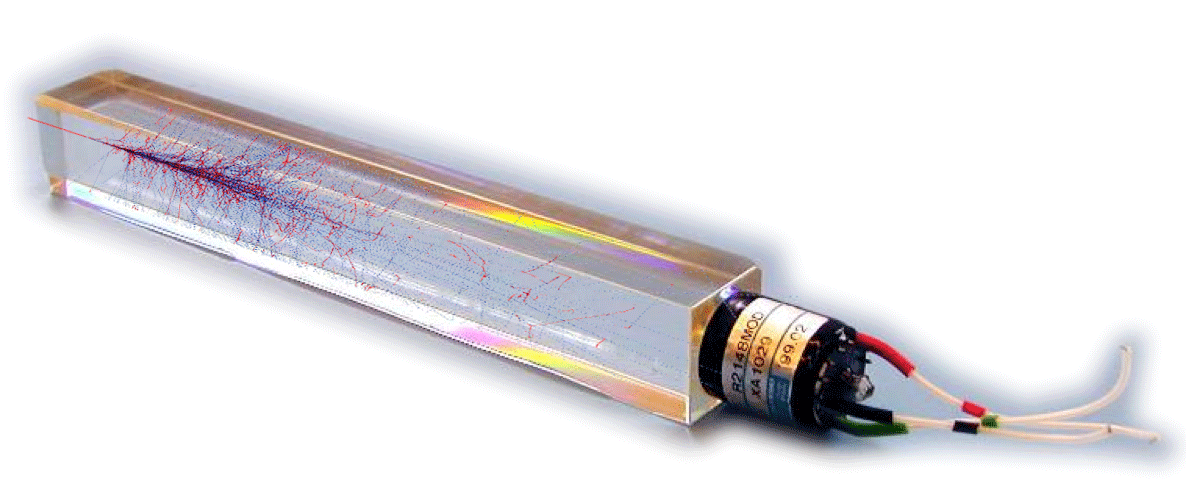
\includegraphics[width=.45\textwidth]{pics/ecal_crystal}
%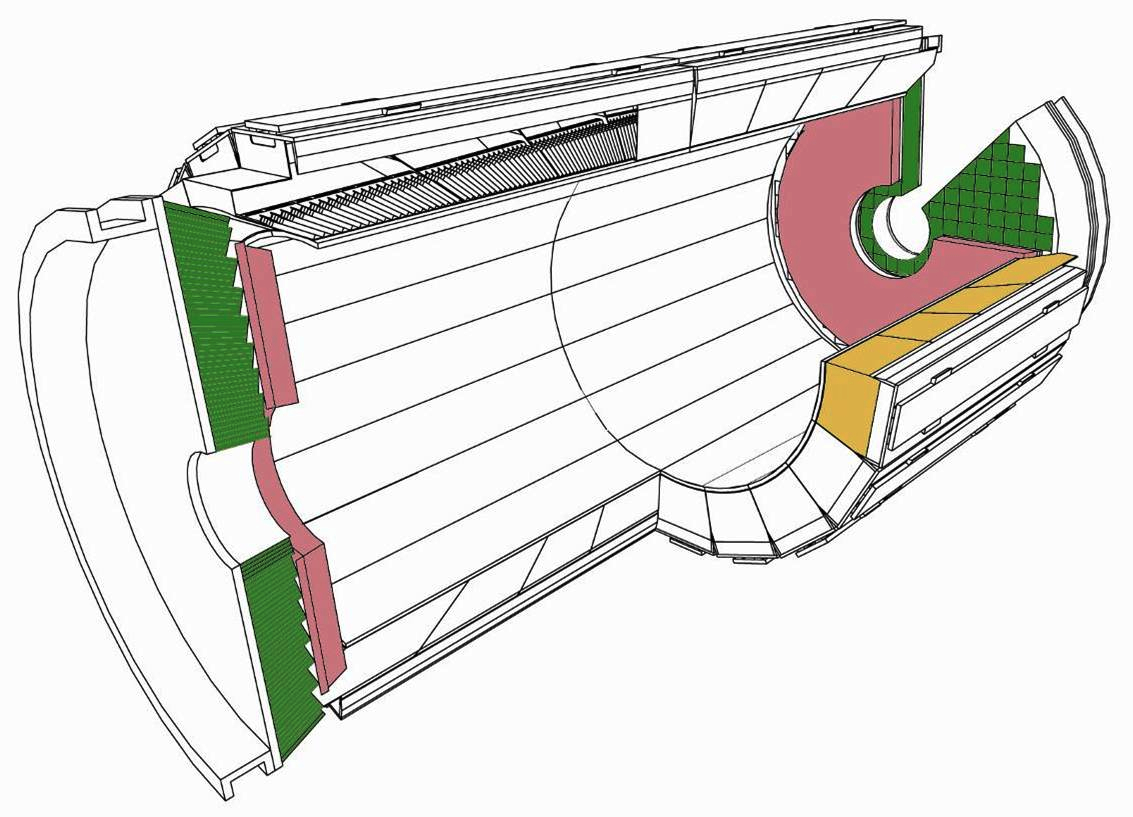
\includegraphics[width=.45\textwidth]{pics/ecal_diagram}
%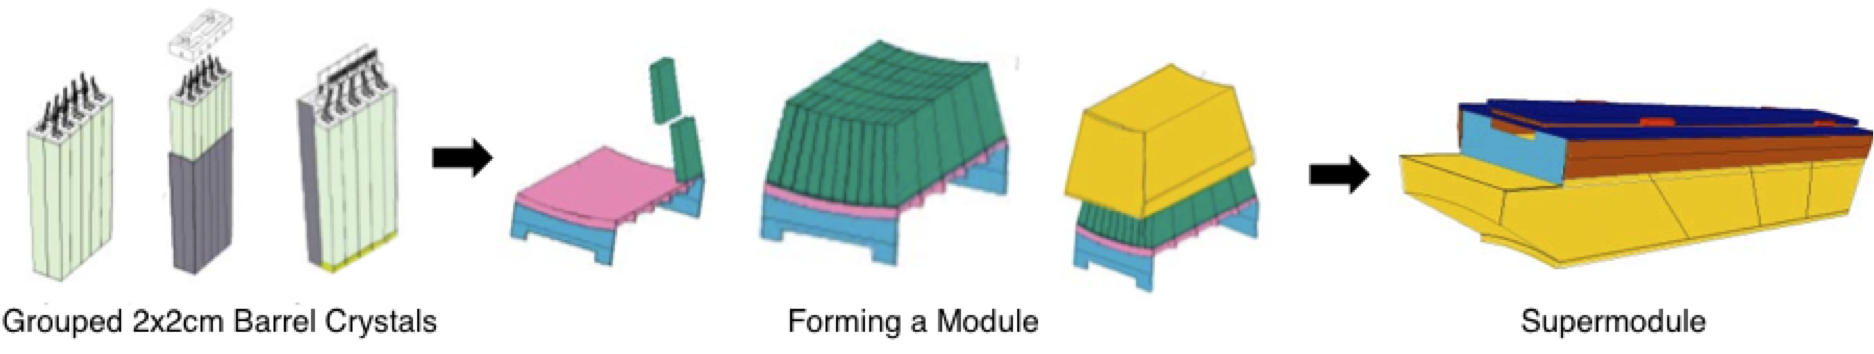
\includegraphics[width=.95\textwidth]{pics/Supermodule}
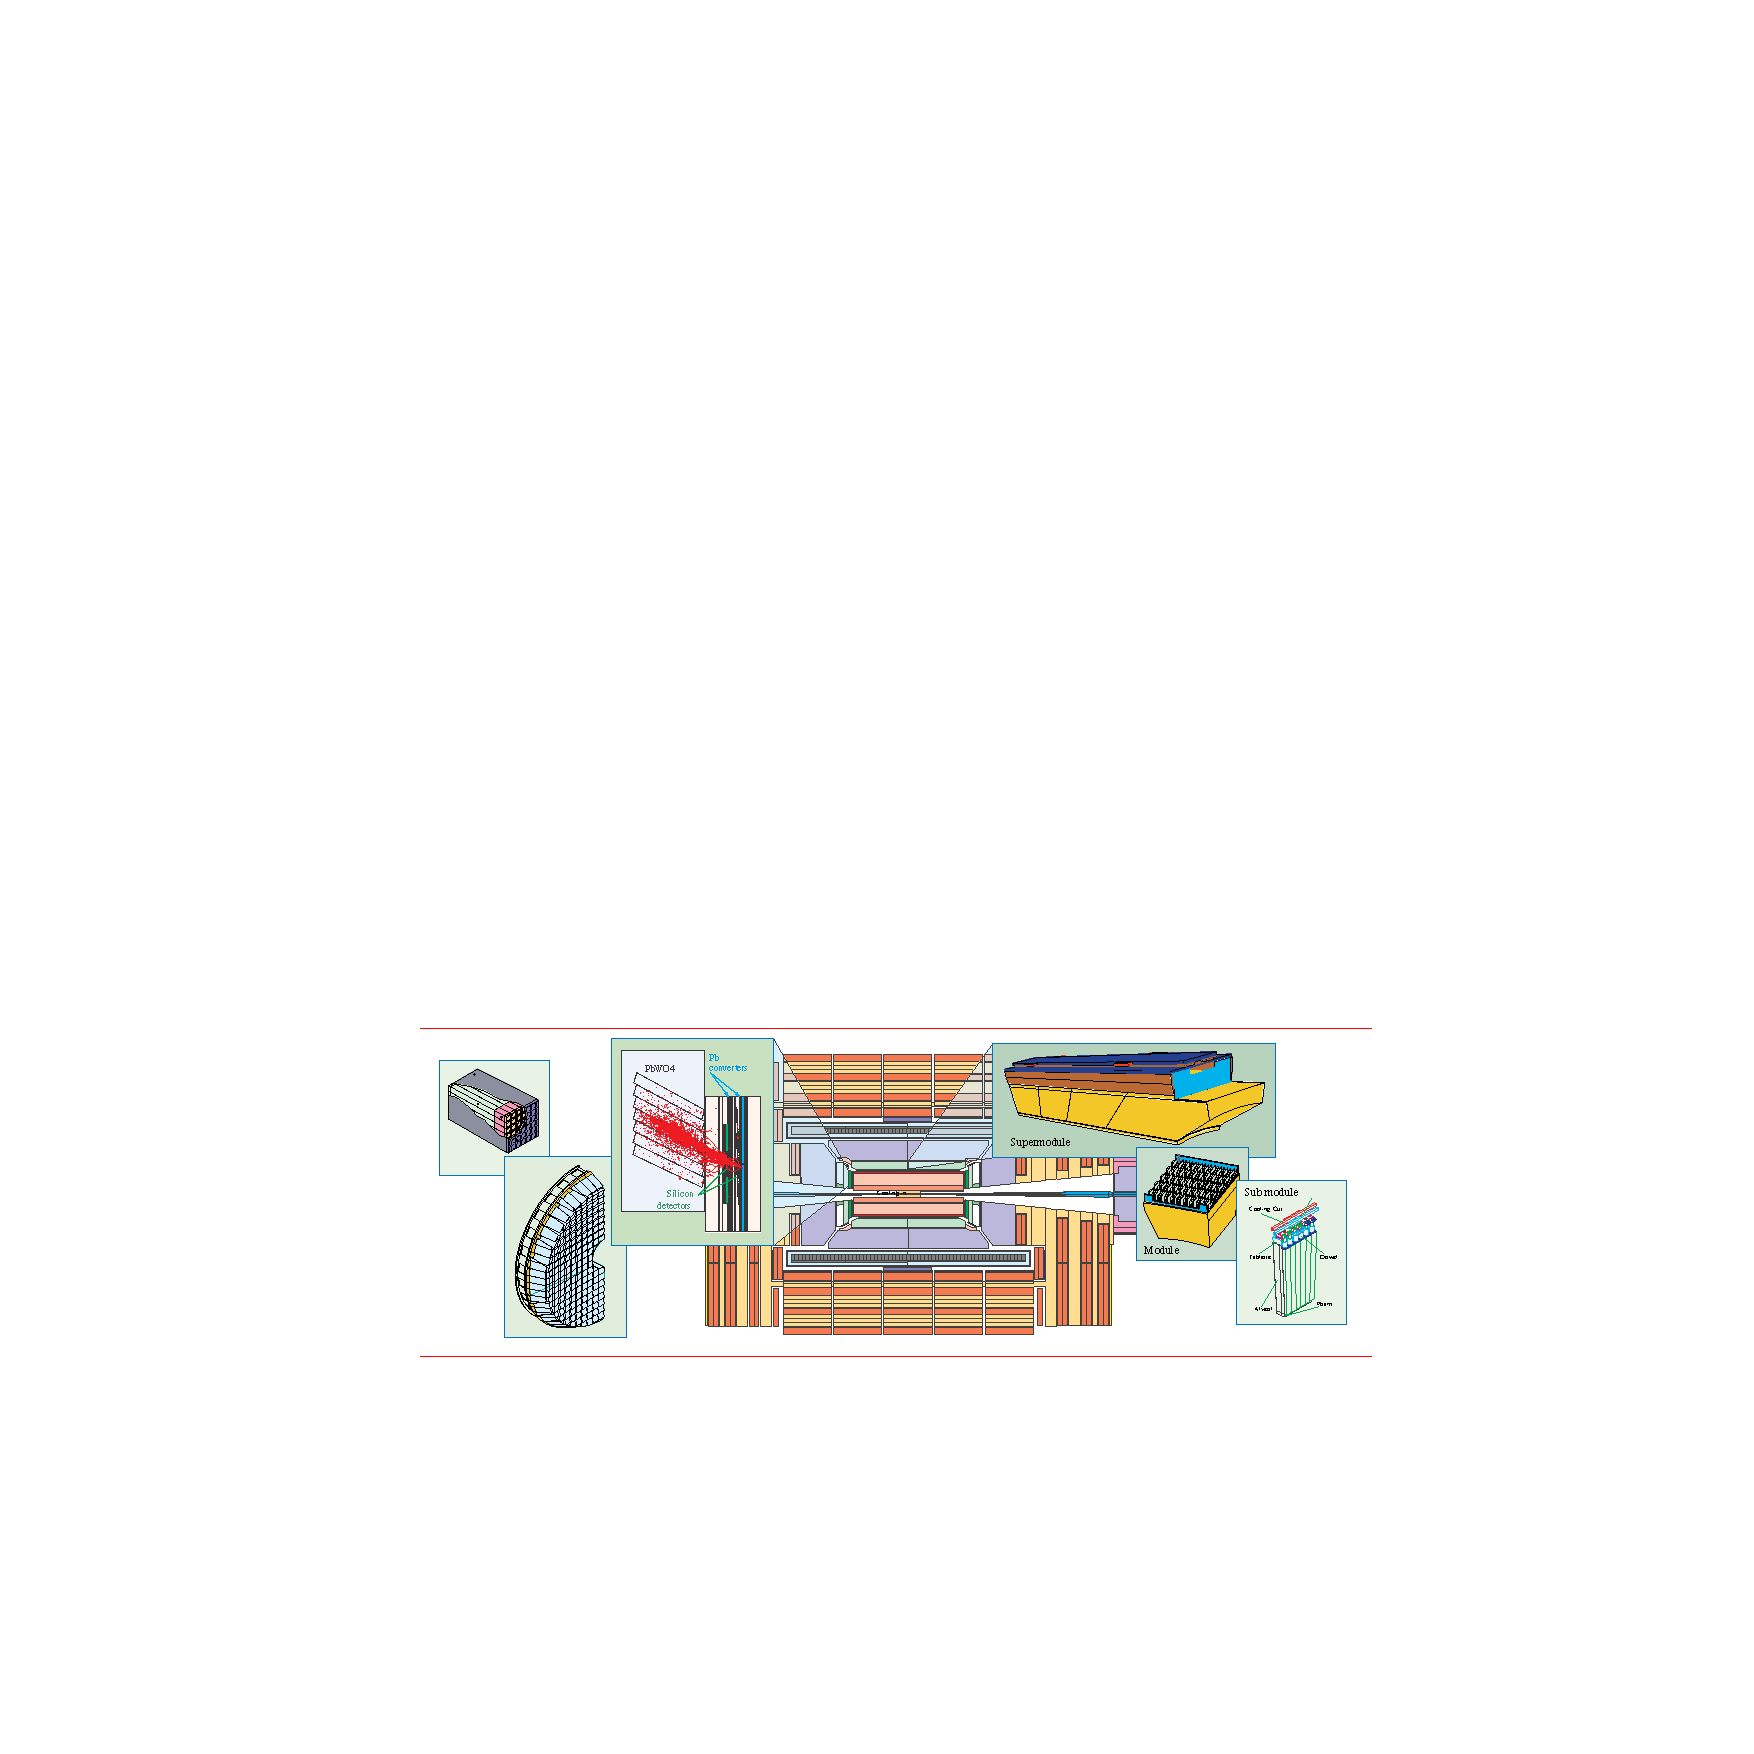
\includegraphics[width=.95\textwidth]{pics/cms_ecal_parts}
\end{center}
\caption{A single CMS ECAL Crystal (top left) tearaway view of distribution of crystals (top right) The construction of a single supermodule (bottom)   }
\label{fig:ecal_cryastal}
\end{figure}

\begin{figure}
\begin{center}
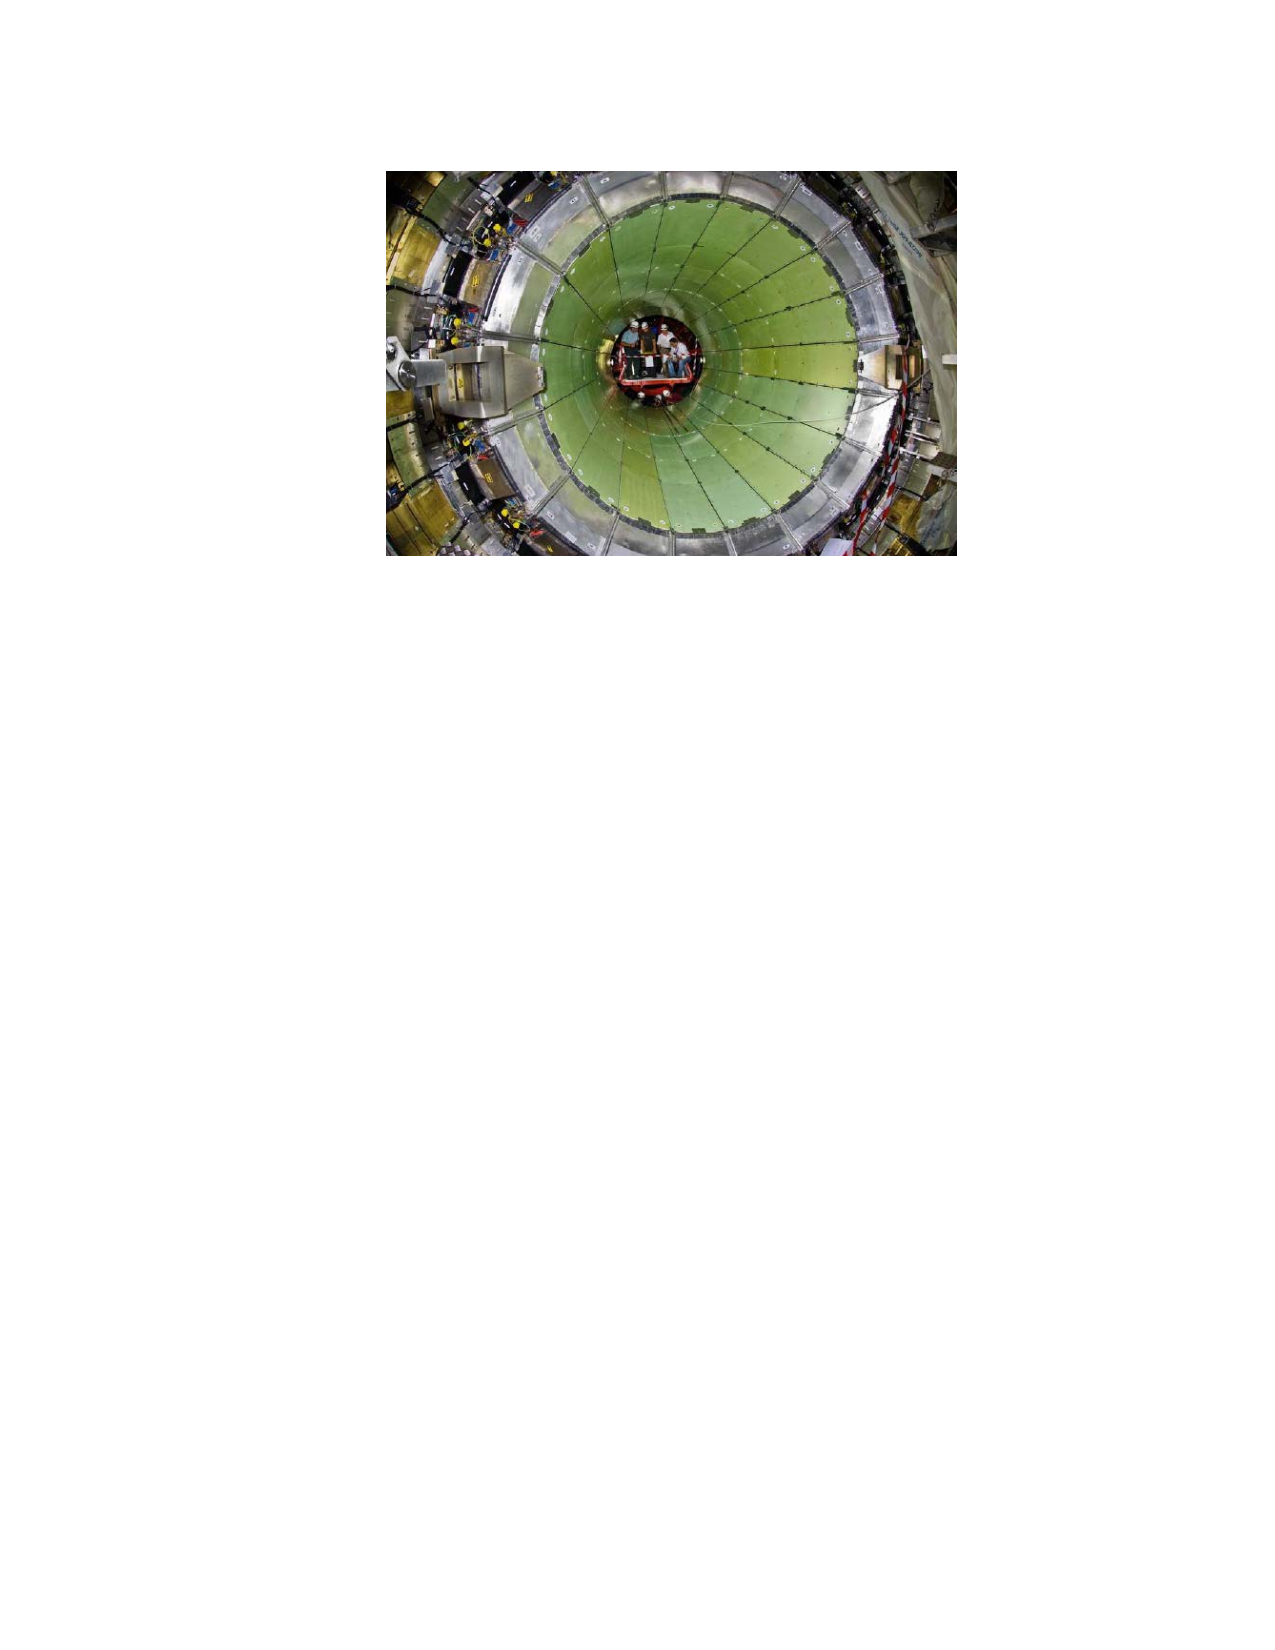
\includegraphics[width=.45\textwidth]{pics/ecal_barrel}
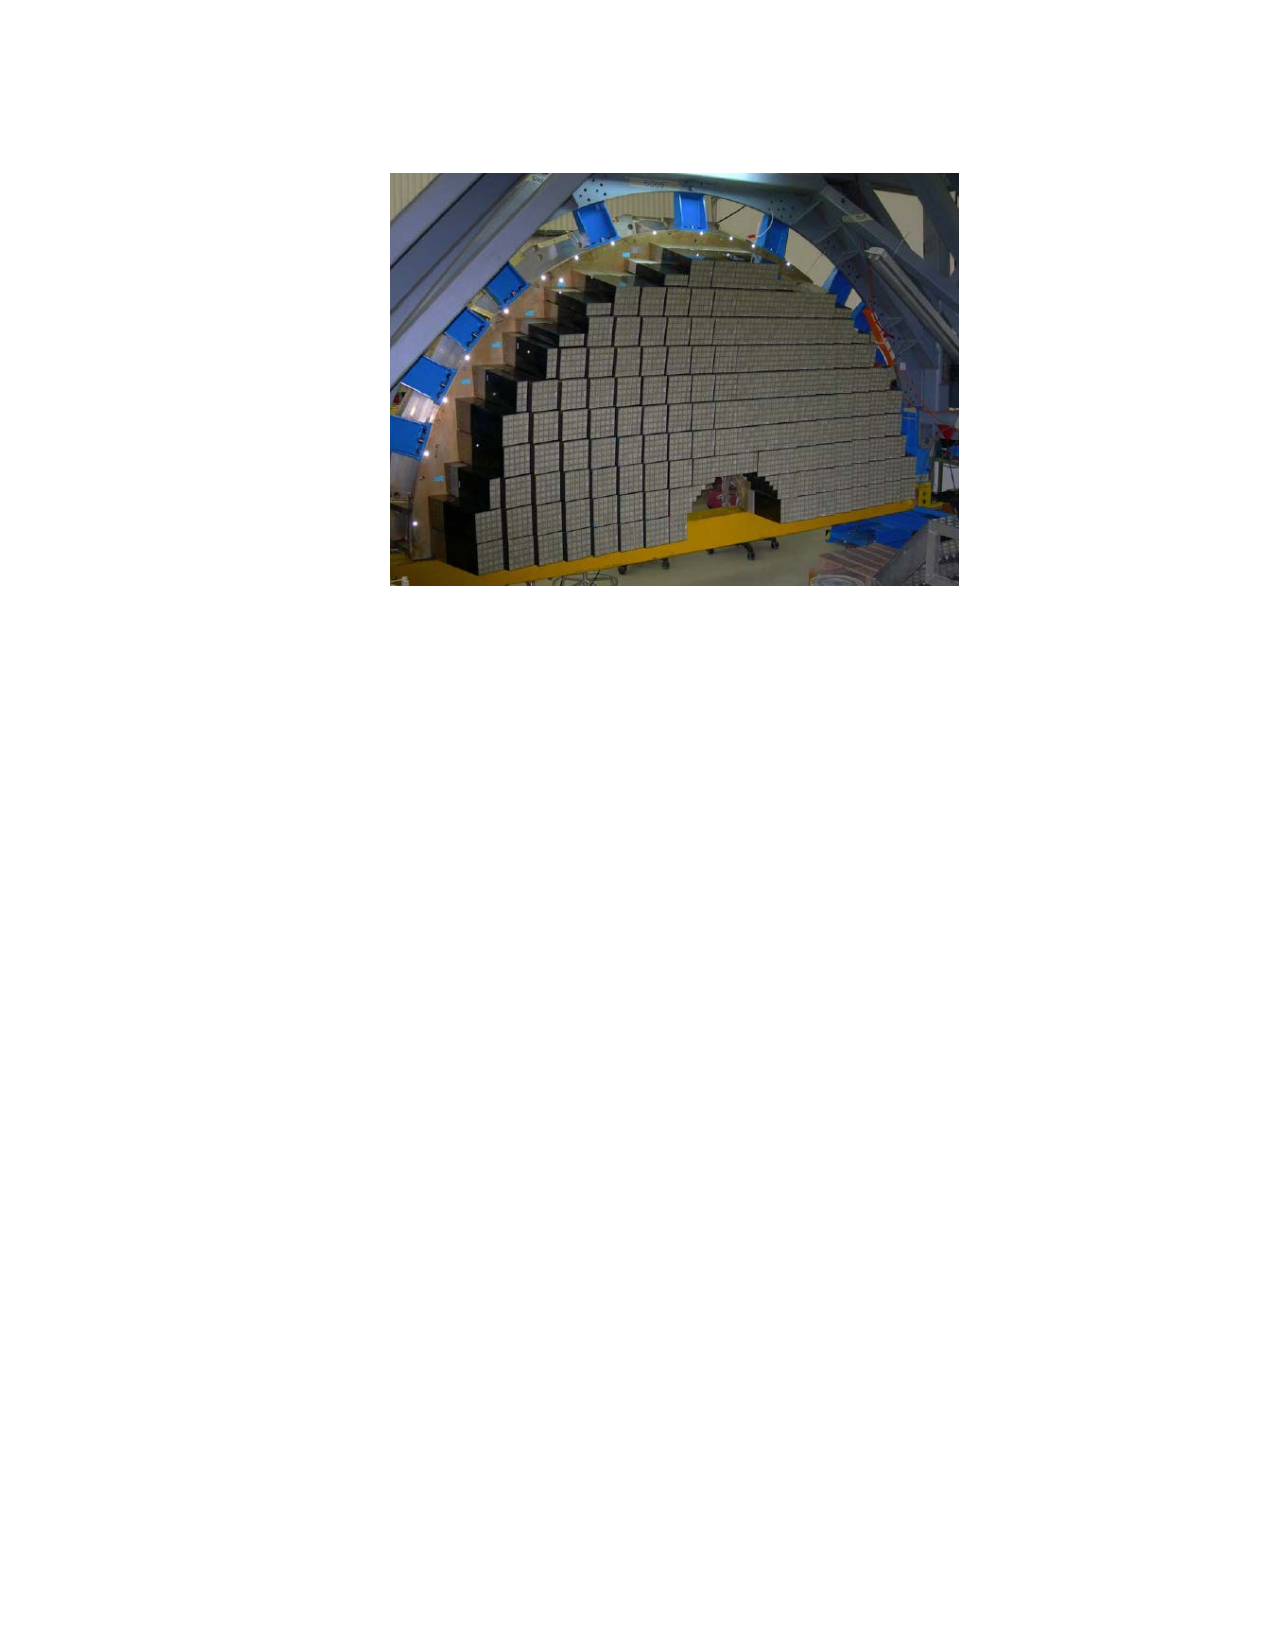
\includegraphics[width=.45\textwidth]{pics/ecal_dee}
\end{center}
\caption{The ECAL barrel installed within CMS (left) A single Dee of the ECAL endcap (right)}
\label{fig:ecal_photos}
\end{figure}

The ECAL consists of 75,848 Lead Tungstate PbWO$_4$ scintillating crystals Fig. \ref{fig:ecal_crystal}. The ECAL is separated into two sections: the Endcaps and the Barrel. 
The Barrel consists of 61200 2x2x23 cm$^3$ crystals separated into 36 Supermodules  and is contained in $|\eta| < 1.48$. The Endcaps are separated into 4 Dees (Fig. \ref{fig:ecal_photos})
 of 3662 crystals with each crystal measuring 3x3x22 cm. 
The 4 dees cover a  pseudorapidity range between $1.48 < |\eta| < 3.0$.
The Endcaps are behind a preshower detector, composed of two lead absorbers 
interleaved with silicon detectors. The preshower covers the pseudorapditiy range
of $1.653 < |\eta| < 2.6$ with each silicon sensor covering a square are of 
63 mm x 63 mm divided into 32 strips. The preshower is designed to give significantly
better spatial resolution than using the endcap alone to aid in the separating single photons
and $\pi^0 \rightarrow \gamma\gamma$ decays used to calibrate the endcap. As the first layer is
2 radiation wavelengths thick such that the majoirty of incident single photons will  
begin to shower before reaching the second layer.  


The preshower converts many of the photons, 
which assists in distinguishing directly produced photons from pairs
of photons resulting from neutral pion decays. 

The light in each crystal is collected as a current 
and amplified by avalanche photodiodes (APDs) in the barrel
region and vaccuum phototriodes (VPTs) in the endcap. This transition is
necessary as the endcap region must be tolerant to much
higher levels of radiation damage from softly scattered (low momentum transfer $Q^2$)
interactions. 

\begin{figure}
\begin{center}
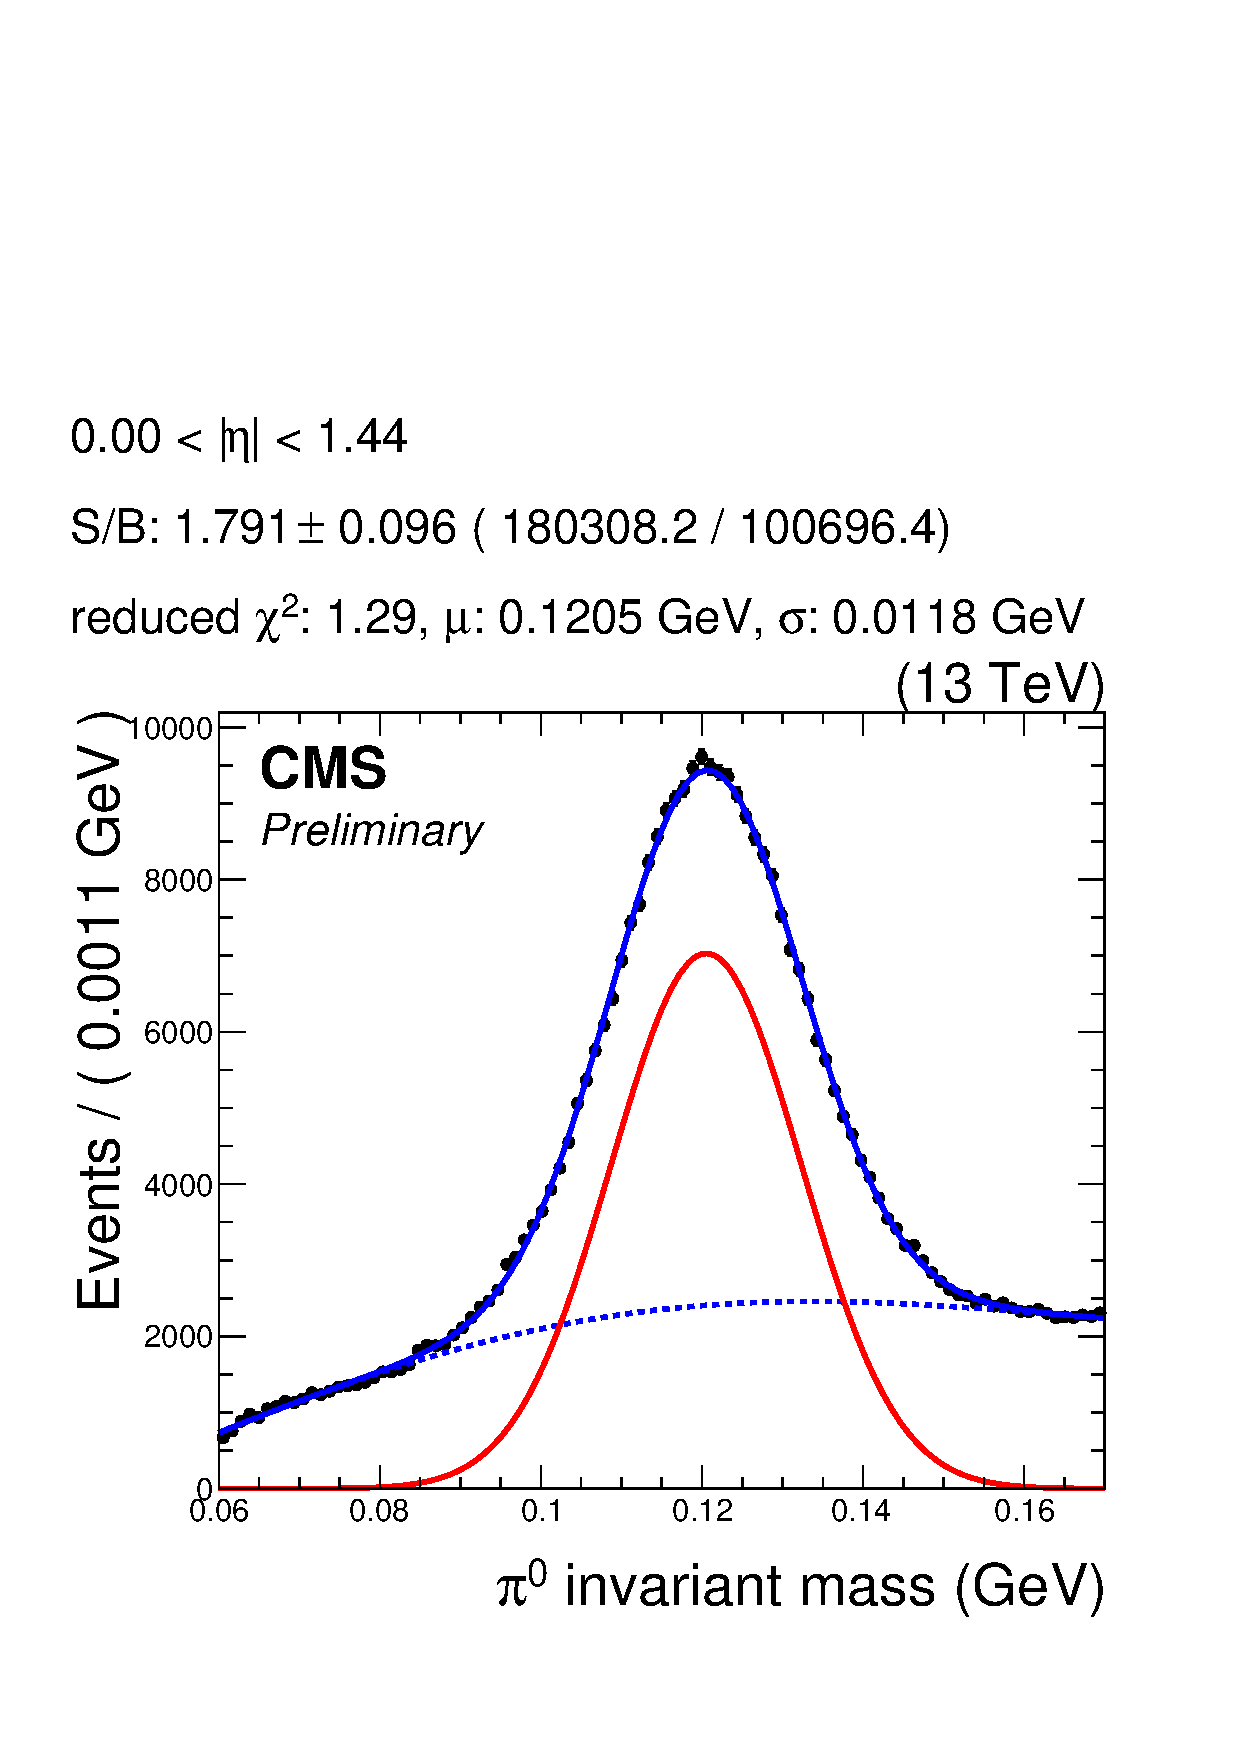
\includegraphics[width=.45\textwidth]{pics/pizero_eb}
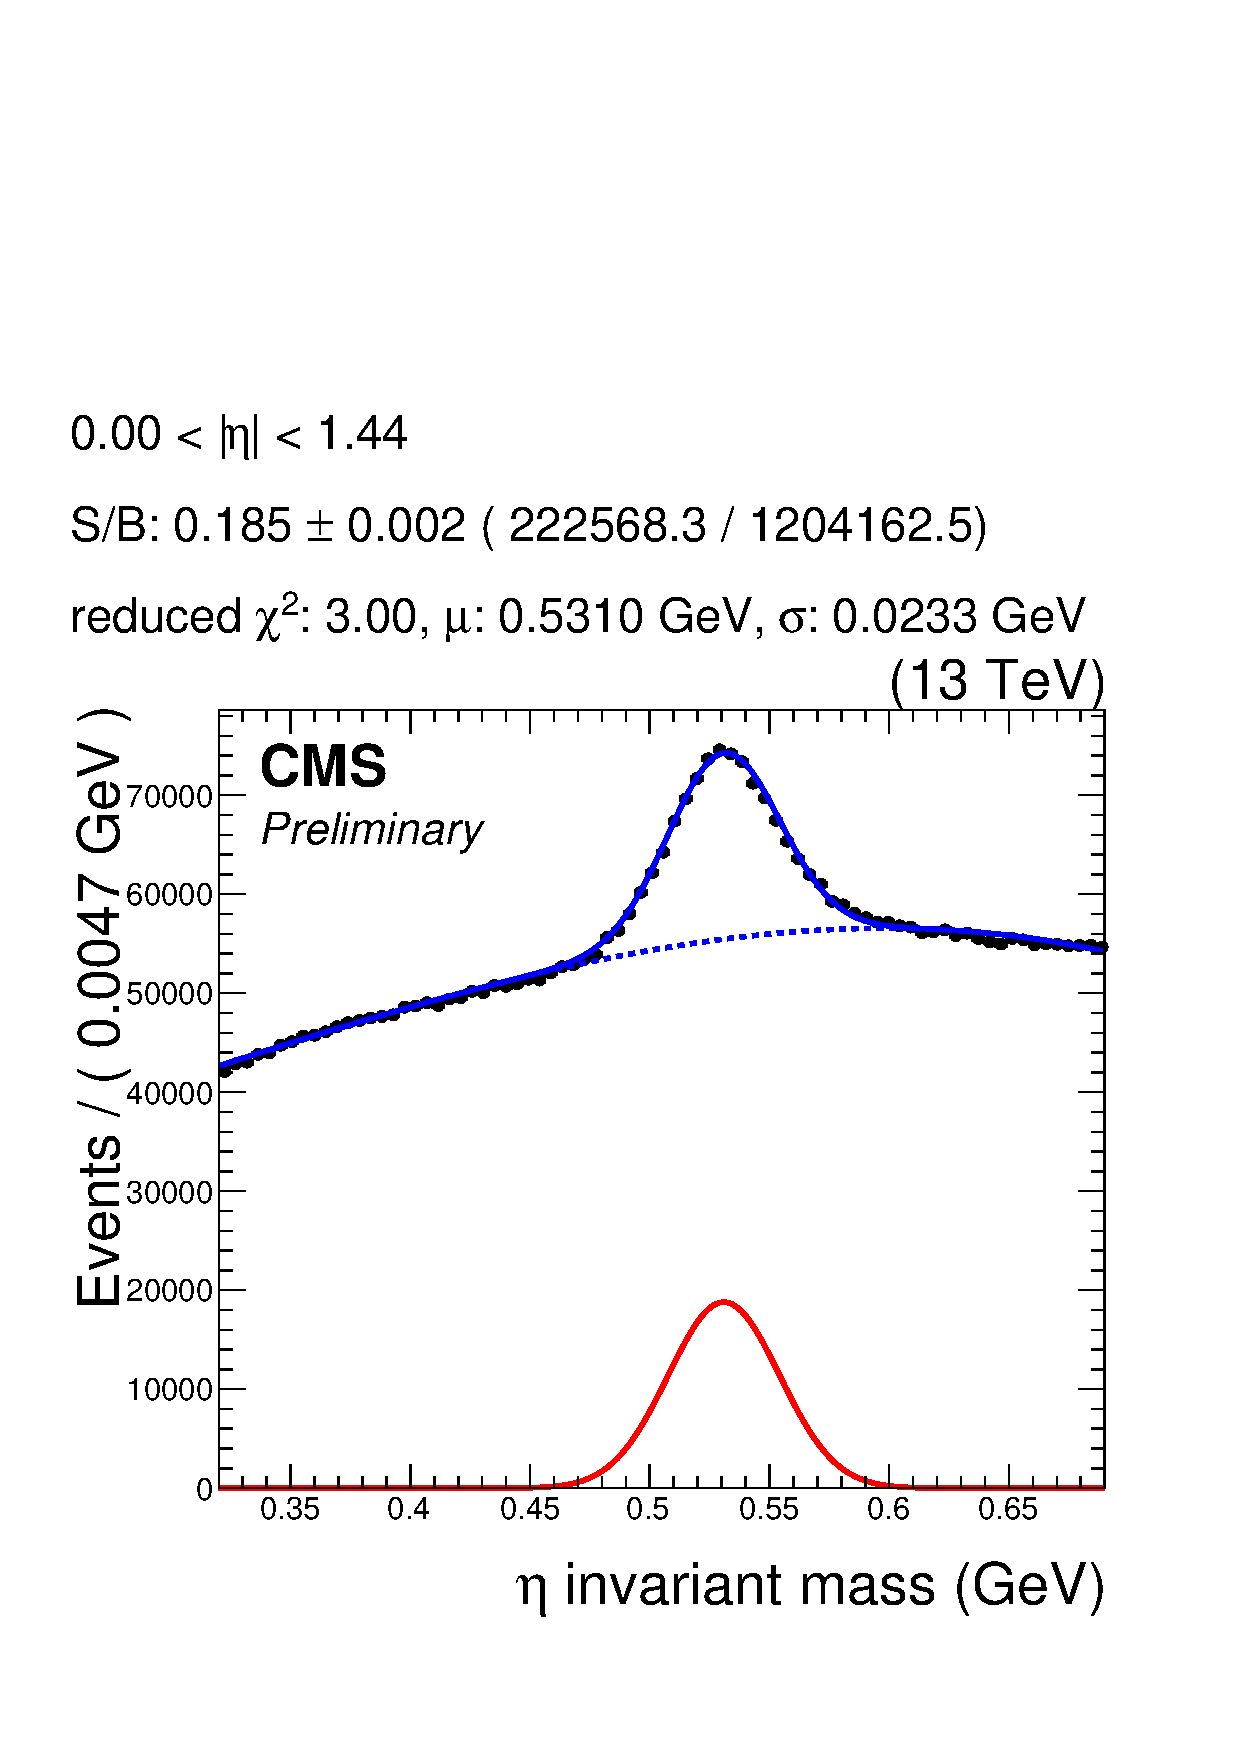
\includegraphics[width=.45\textwidth]{pics/eta_eb_2015b}
\end{center}
\caption{Calibration stream outputs for the pizero and eta barrel trigger paths}
\label{fig:pizero_eta}
\end{figure}

The detector is calibrated with a method that reconstructs the mass of neutral
pion and eta-mesons to precisely calibrate the entire ECAL. The copious
production of these particles in hadronic jets at the LHC allows us to
perform this calibration rapidly, even at very low luminosity.

Under irradiation, the crystals undergo transpancy changes 
due to the formation of color centers, which interestingly recover spontaneously when there
is no radiation present. As the crystal transparency affects the energy measurent,
the crystal transparency is continuoulsy monitored by a laser monitoring system. 
The system takes advantage of a 3 $\mu$s gap in the LHC bunch train to inject the
pulses at a rate of 100 Hz. This rate allows for a measurement of every crystal
to be made at least every 30 minutes. In the barrel, only laser
 pulses of known wavelength are injected through optical fibers. In the endcap, LEDs provide
an additional wavelength. 

The presence of the preshower also causes some degradation of the
Endcaps' energy resolution relative to the Barrel. 



\section{Hadronic Calorimeter (HCAL)}

\begin{figure}
\begin{center}
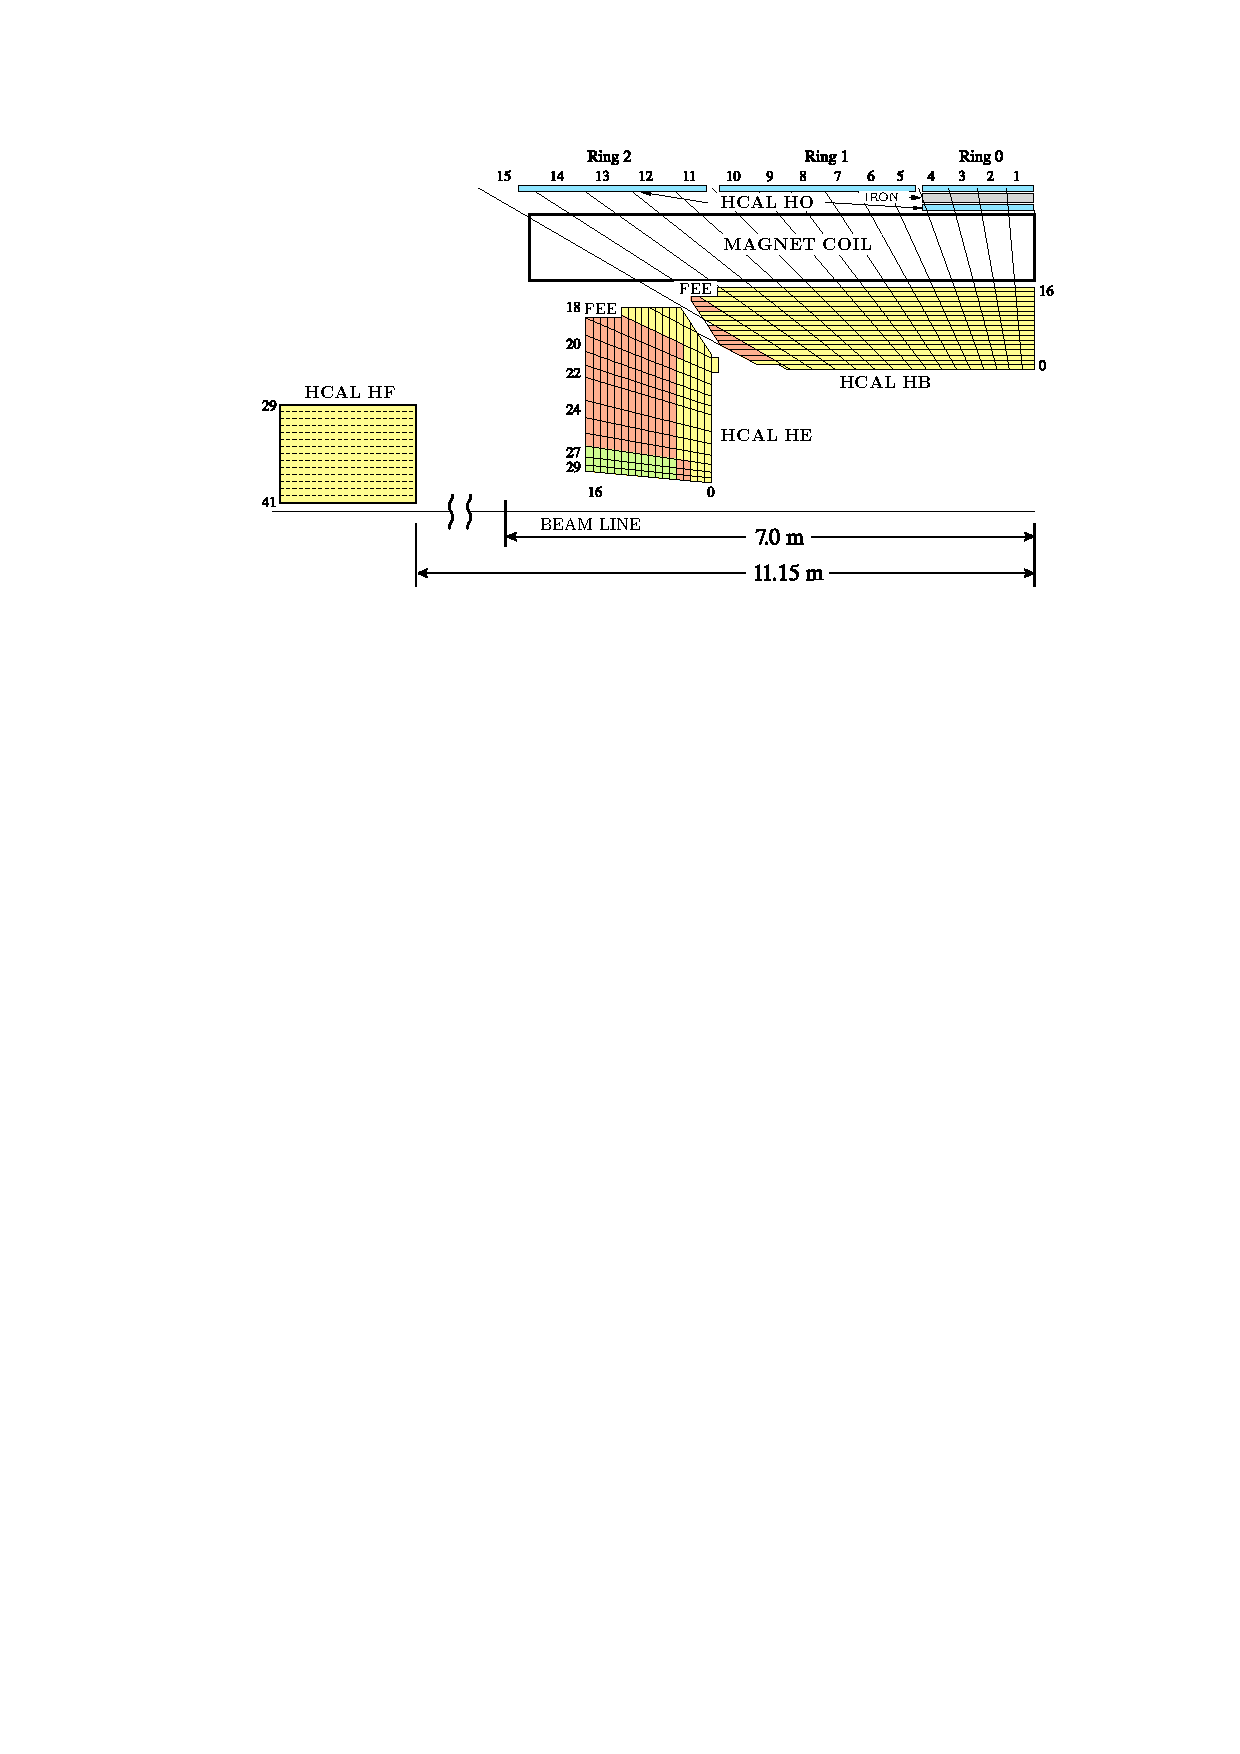
\includegraphics[width=.95\textwidth]{pics/hcal_diagram}
\end{center}
\caption{Kinematic acceptance of the CMS HCAL}
\label{fig:hcal_diagram}
\end{figure}

\begin{figure}
\begin{center}
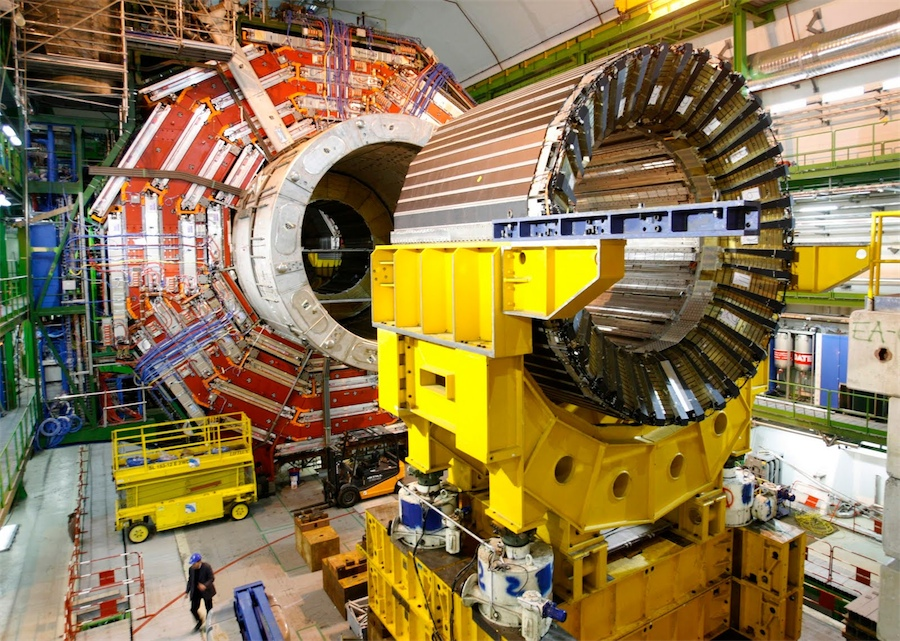
\includegraphics[width=.65\textwidth]{pics/naked_hcal}
\end{center}
\caption{The CMS HCAL outside of the detector}
\label{fig:hcal_naked}
\end{figure}


Surrounding the ECAL. The Hadronic Calorimeter (HCAL) is hermetic (full coverage of interaction), non-compensating (asymmetric eletromagnetic and hadronic energy response), sampling calorimeter (showering material differs from measurment material) designed to measure the the energy of neutral hadrons which would not deposit significant energy in the ECAL. 

 The ratio of energy between the two detectors for defined solid angle, $H/E$, is a 
commonly used particle identification criterion. 

The HCAL consists of 9072 channels divided between four sections: the barrel (HB), the endcap (HE), 
two forward calorimeters (HF) and an outer hadron calorimieter (HO). The barrel
 and endcap of the HCAL cover $|\eta| < 4$. The forward detectors extend the subdetector's reach to $|\eta| =5$. 
As the HCAL is radially limited by the design of the enclosing solenoid, 
the HO is built around the solenoid to measure any leaked energy from high momentum showers. The towers are segmented into towers that project into $\eta,\phi$ space with $\Delta \eta \times\delta \phi= 0.087 \times 0.087$ for $|\eta| < 1.6$ and 
$\Delta \eta \times\delta \phi= 0.17 \times 0.17$ for $|\eta| > 1.6$. 

The HF subdetector is a cherenkov light detector using quartz fibers within 165 cm of steel absorber. 
Photomultiplier tubes (PMTs) connected to the fibers convert the detected light to a detectable signal. Cherenkov detectors
 utilize the characteristic electromagnetic ``sonic boom'' created by particles traveling faster than light can travel in
 a material. As the angle of emission and intensity of the radiation depends on the velocity of the particle. For energetic
particles $E>1$ GeV the energy lost to the radiation is negligble (cite-the-physics-of-particle-detectors-book).

Unlike electromagnetic showers, hadronic interaction cross sections are an order of magnitude smaller for the same material. To compensate cost effectively, hadronic calroimeters are constructed from dense materials usch as copper,
 iron, lead, uranium, and tungsten (cite-tully). In general, hadronic showers produce irregularly 
shaped deposits and varied particle content when compared to electromagnetic showers. 
 
\begin{figure}
\begin{center}
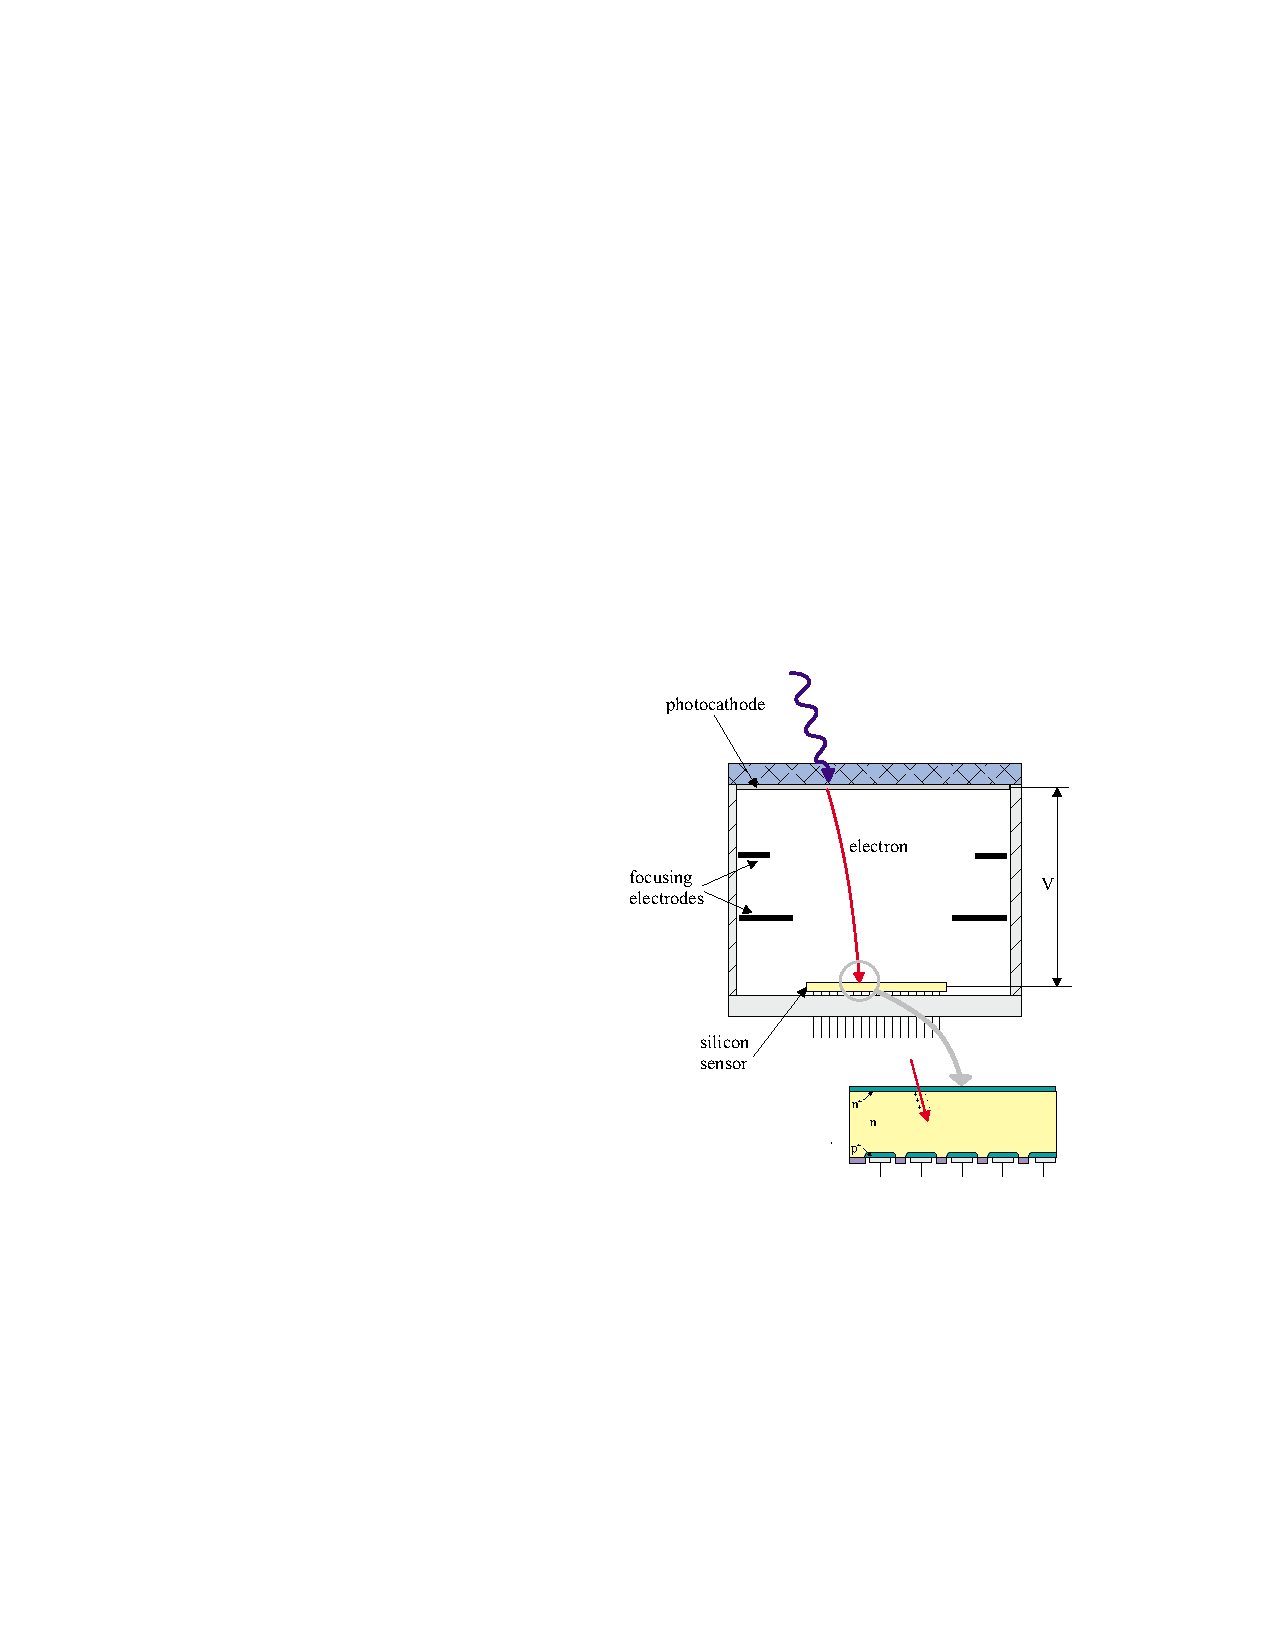
\includegraphics[width=.45\textwidth]{pics/HPD}
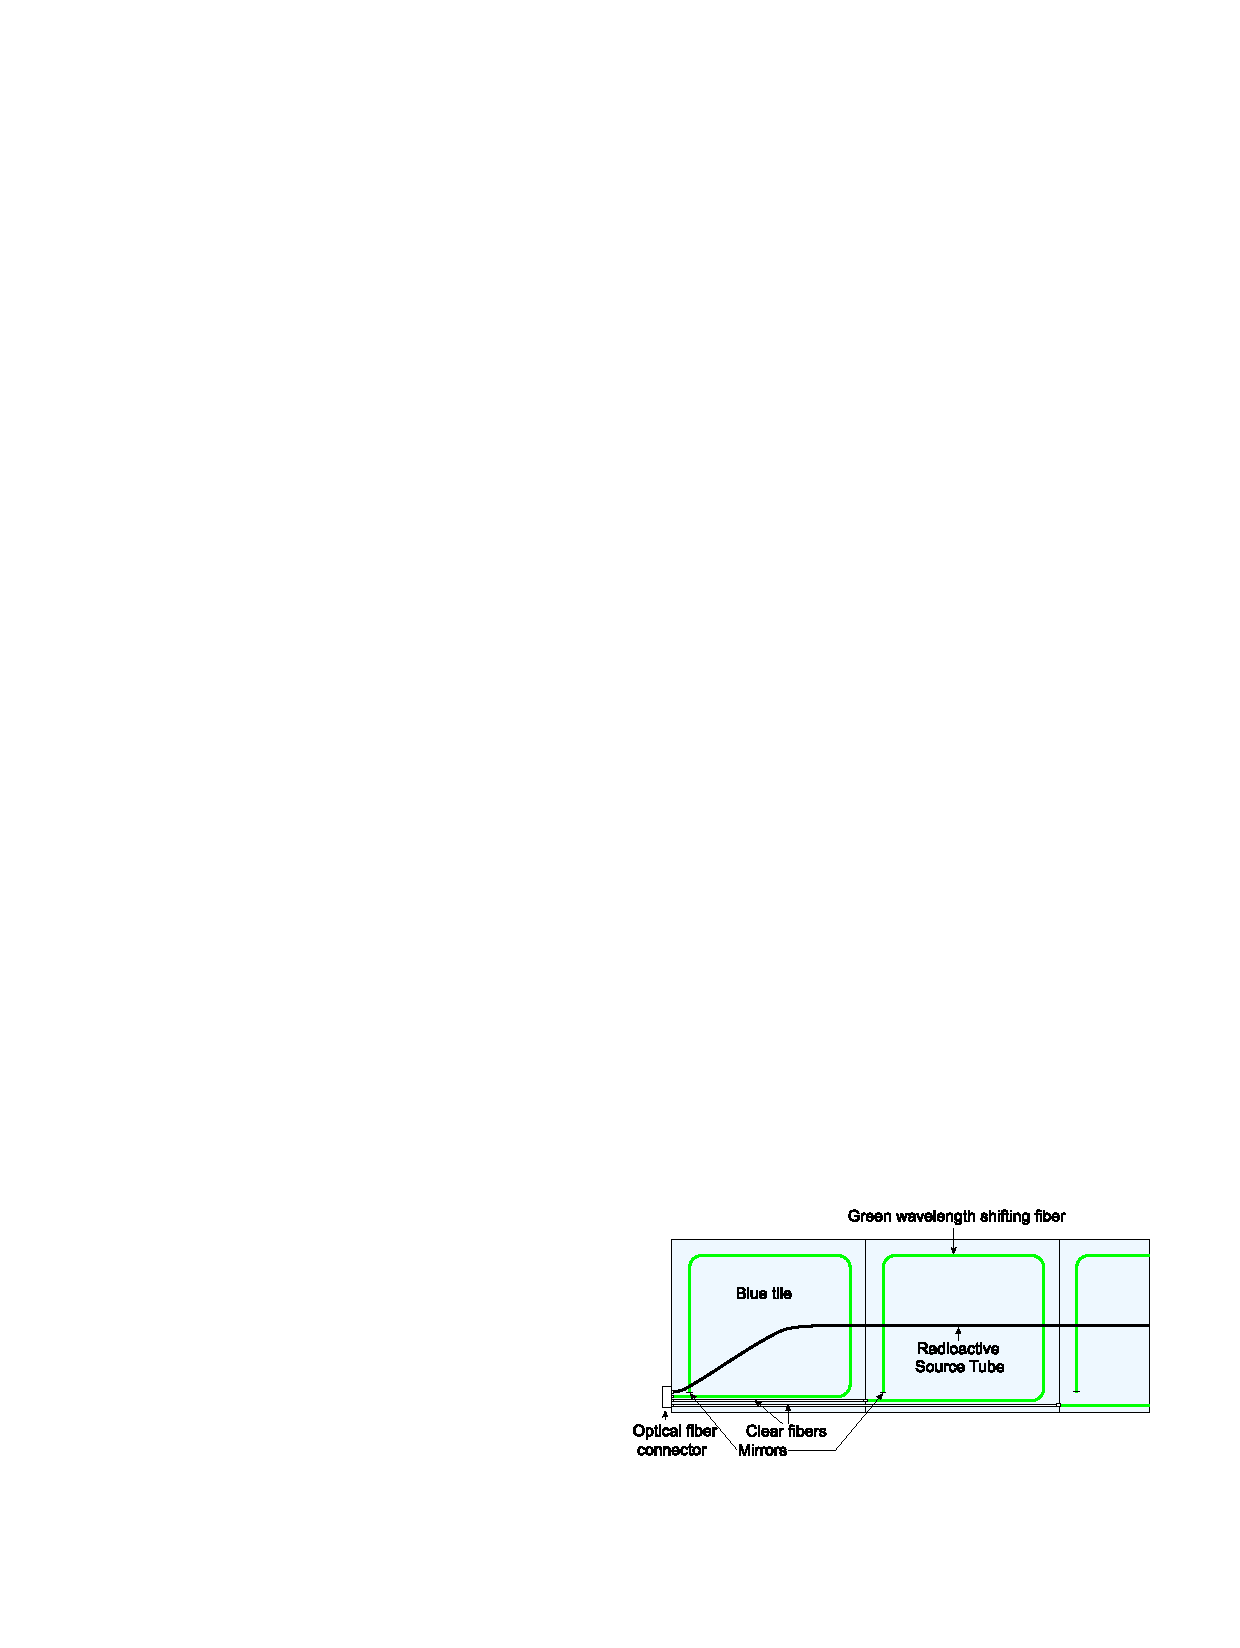
\includegraphics[width=.45\textwidth]{pics/HCALfiber}
\end{center}
\caption{(Left) Diagram of a typical HPD under a potential difference $V$ (cite-hpd-cern) (Right) 2 visible scintillator 
plates of 16 (cite-hcal-calib)}
\label{fig:hpd_fiber}
\end{figure}

\begin{figure}
\begin{center}
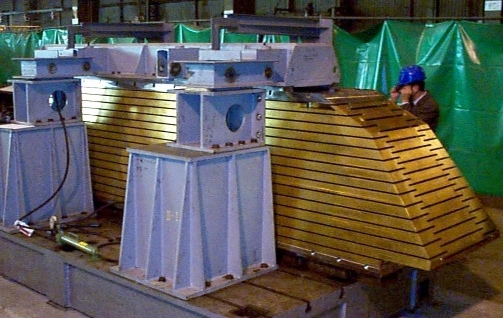
\includegraphics[width=.45\textwidth]{pics/hb_wedge}
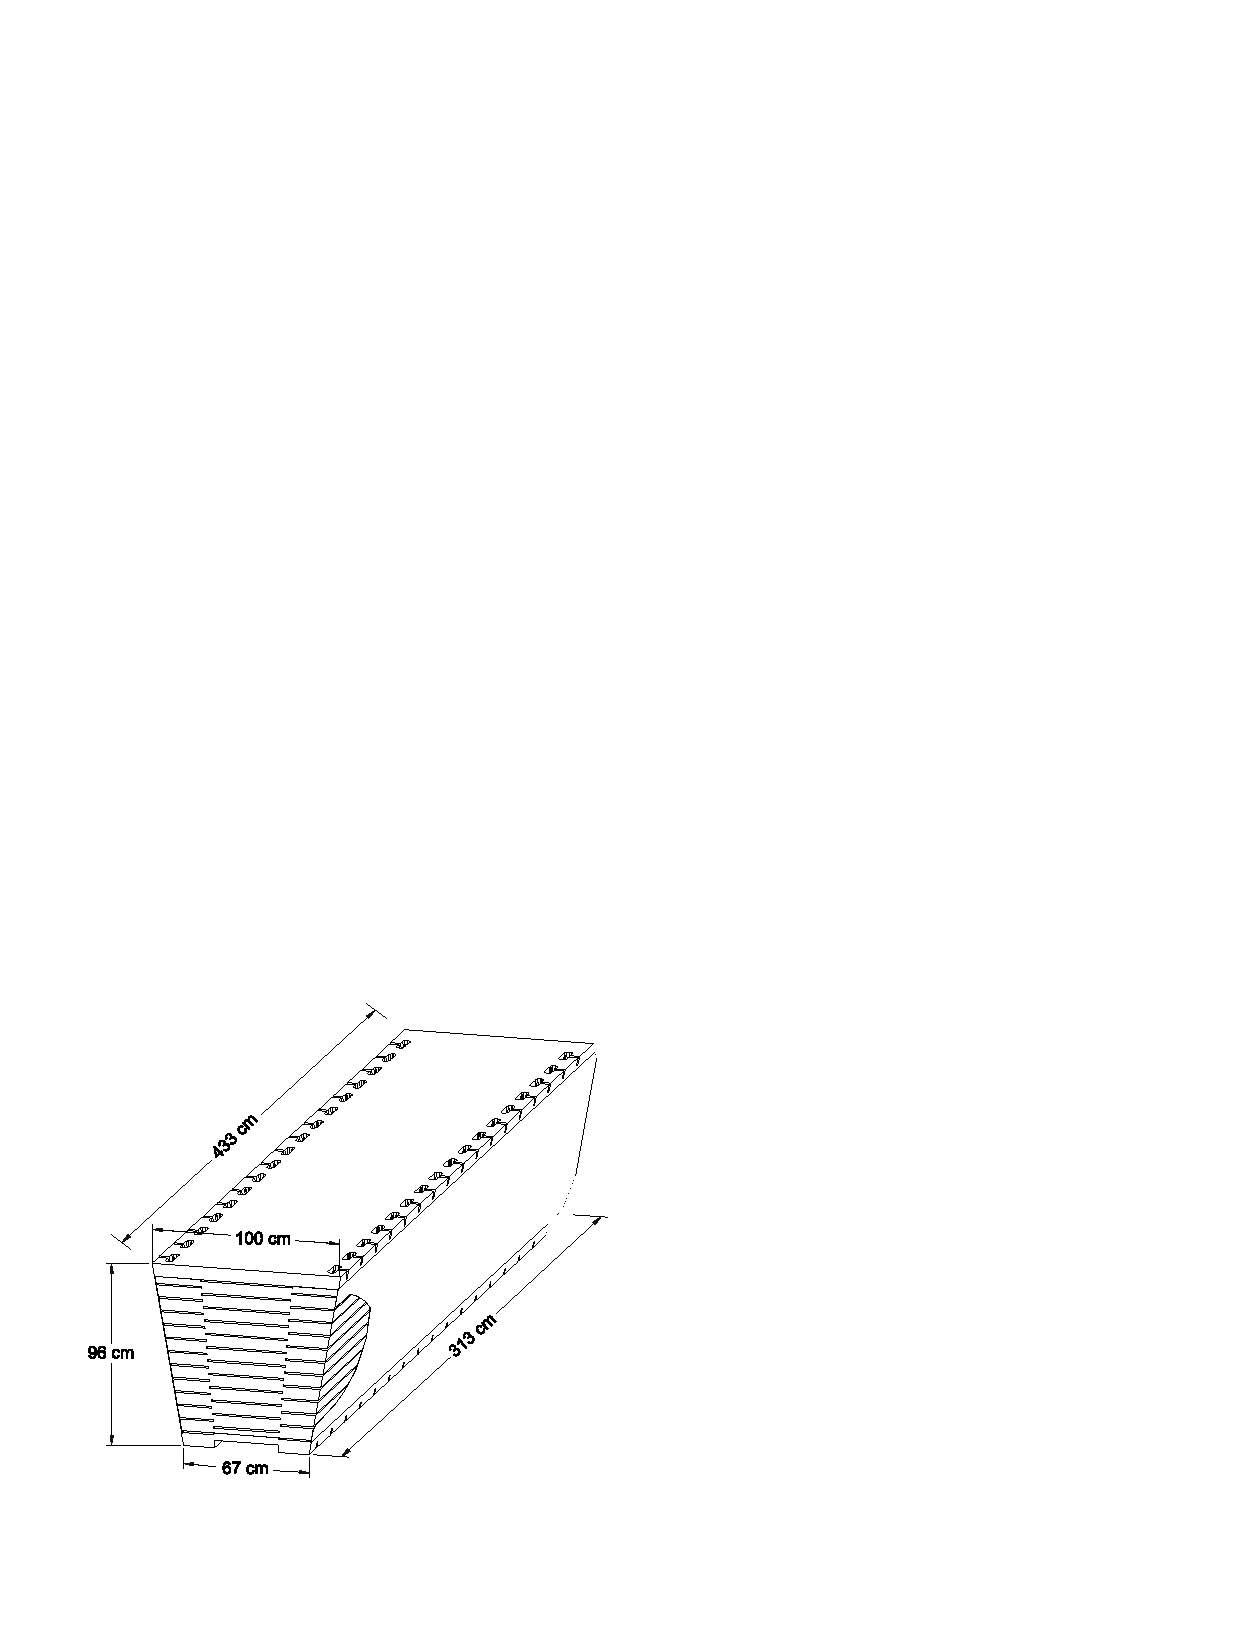
\includegraphics[width=.45\textwidth]{pics/HBwedge}
\end{center}
\caption{(Left) A single wedge of the CMS HCAL barrel (Right) Scintillator trays \ref{fig:hpd_fiber} are inserted into slots at the end of the wedge (cite-hbcalib)}
\label{fig:hb_wedge}
\end{figure}

The detector is constructed as alternating layers of brass absorber and plastic scintillator. 
The light is merged, wavelength shifted and measured by hybrid photodiodes (HPDs) with 17 channels per HPD. The HPD
(Figure \ref{fig:hpd_fiber}) functions by converting light into photoelectrons emitted at the photocathode and accelerated
by a potential difference of 8-10 kV toward the silicon layer. The absorbed energy in the silicon sensor induces 
electron hole pairs which induce a detectable current. The light is wavelength shifted to avoid a loss in photons 
when piping light to the HPDs through a small cross sectional fiber. We are able to evade phase space 
conservation (photon flux per unit area) by redefining the phase space element in a lower energy wavelength specturm.  {

Large deposits of energy reconstructed as purely hadronic energy in the HCAL is of particular interest 
to the study of long lived decays when the long-lived decay occurs inside of the HCAL calorimetetry. Although not studied here,
large signal to background discrimination can be found by requiring a calorimeter deposit to have no
associated tracks and a large ratio of hadronic energy $H/E$. It is also of concern that the HCAL is known to report
 have spurious noise that generally result in the mis-measurement of missing energy, but would mimics the signature
of long lived decays. It is possible that using a coincidence of acitivity in the muon spectromoeter could supressed 
these events.  

\section{Tracking Layers}

\begin{figure}
\begin{center}
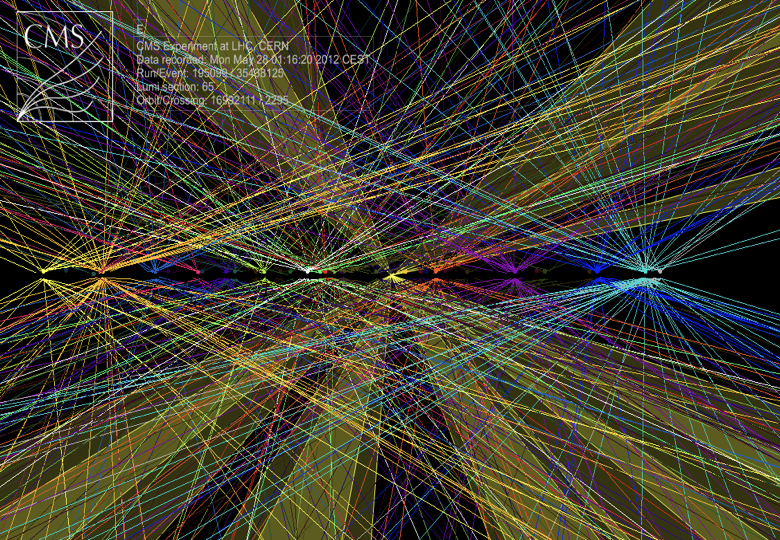
\includegraphics[width=.75\textwidth]{pics/pileup_vertices}
\end{center}
\caption{Pileup Interactions}
\label{fig:pileup}
\end{figure}

The CMS tracker's purpose is to reconstruct the trajectories (or simply ``tracks'') of the charged particles
 copiously produced in hadron collisions. Using knowledge of the magnetic field along trajectory
 with position measurements taken from multiple layers of silicon strips and pixels, the helicoidal tracks are
 fit and kinematic parameters extracted.  

A charged particle in a uniform magnetic field (like that of the CMS Solenoid) 
are parameterized by 5 parameters:
\begin{itemize}
\item $d_{\rho}$: the distance of closest approach to the reference point
\item $\phi_0$: azimuthal angle specifying the reference point to the helix center 
\item  $p_t^*$: charged signed transverse momentum
\item  $d_z$: signed distance of the helix from the reference point in the z direction
\item $\tan \lambda$: the slope of the track 
\end{itemize}
using these parameters, the trajectory is parameterized in the turning angle $\phi$:
\begin{align*}
x =& x_0 + d_\rho \cos \phi_0 + \alpha p_{t}^* ( \cos \phi_0 - \cos(\phi_0 + \phi) ) \\
y =& y_0 + d_\rho \sin \phi_0 + \alpha p_{t}^* ( \sin \phi_0 - \sin(\phi_0 + \phi) ) \\
z =& z_0 + d_z - \alpha p_{t}^*  \tan \lambda \cdot \phi 
\end{align*}
It is important to note that tracks do not necessarily  have the same reference point. For CMS, each
individual track parameter is computed against a reference point determined by the the closest
point of approach to the beamline. For prompt physics, this reference point coincides with the
collision vertex used to compute the kinematic parameters for calorimeter jets. In contrast, when
tracks are displaced, the reference point used for the track is not the same as the reference point
for the calorimeter jet $eta$ and $\phi$. This mis-match of coordinate systems affects the ultimate
track and jet association. 

By fitting trajectories to vertices the tracker enables the reconstruction 
of the hard interaction position (Figure \ref{fig:pileup}). As only one vertex is typically
of interest, identifying background vertices and subtracting their contribution is of increasing
importance with the increasing instantaneous luminosity. 

As photons and electrons exhibit nearly identical signatures in the ECAL, the reconstruction of the
track associated to electrons is of particular interest.

\begin{figure}
\begin{center}
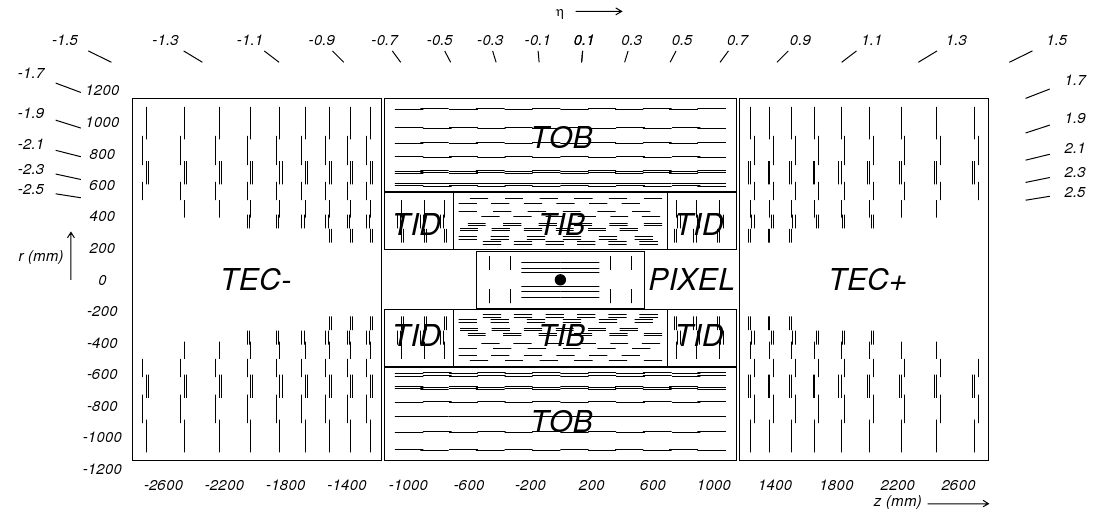
\includegraphics[width=.95\textwidth]{pics/tracker_diagram}
\end{center}
\caption{Kinematic acceptance of the CMS tracker}
\label{fig:tracker_diagram}
\end{figure}

The CMS tracker is the worlds largest all silicon detector with a
 sensitive area larger than 200 m$^{2}$ (Figure \ref{fig:tracker_strips_and_module}) (cite-2014-tracker-performance). 
The tracker consists of 10 layers
in the barrel region: 4 inner barrel layers (TIB) and 6 outer barrel layers (TOB). The endcap is made up of 
12 disks: 3 inner disks (TID) and 9 endcap disks (TEC). 


\begin{figure}
\begin{center}
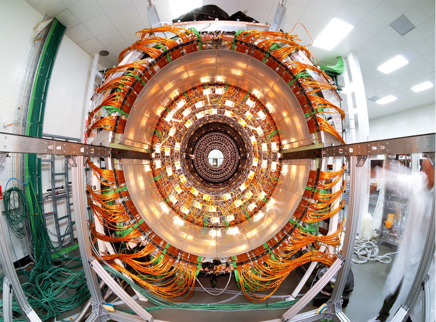
\includegraphics[width=.45\textwidth]{pics/naked_pixel}
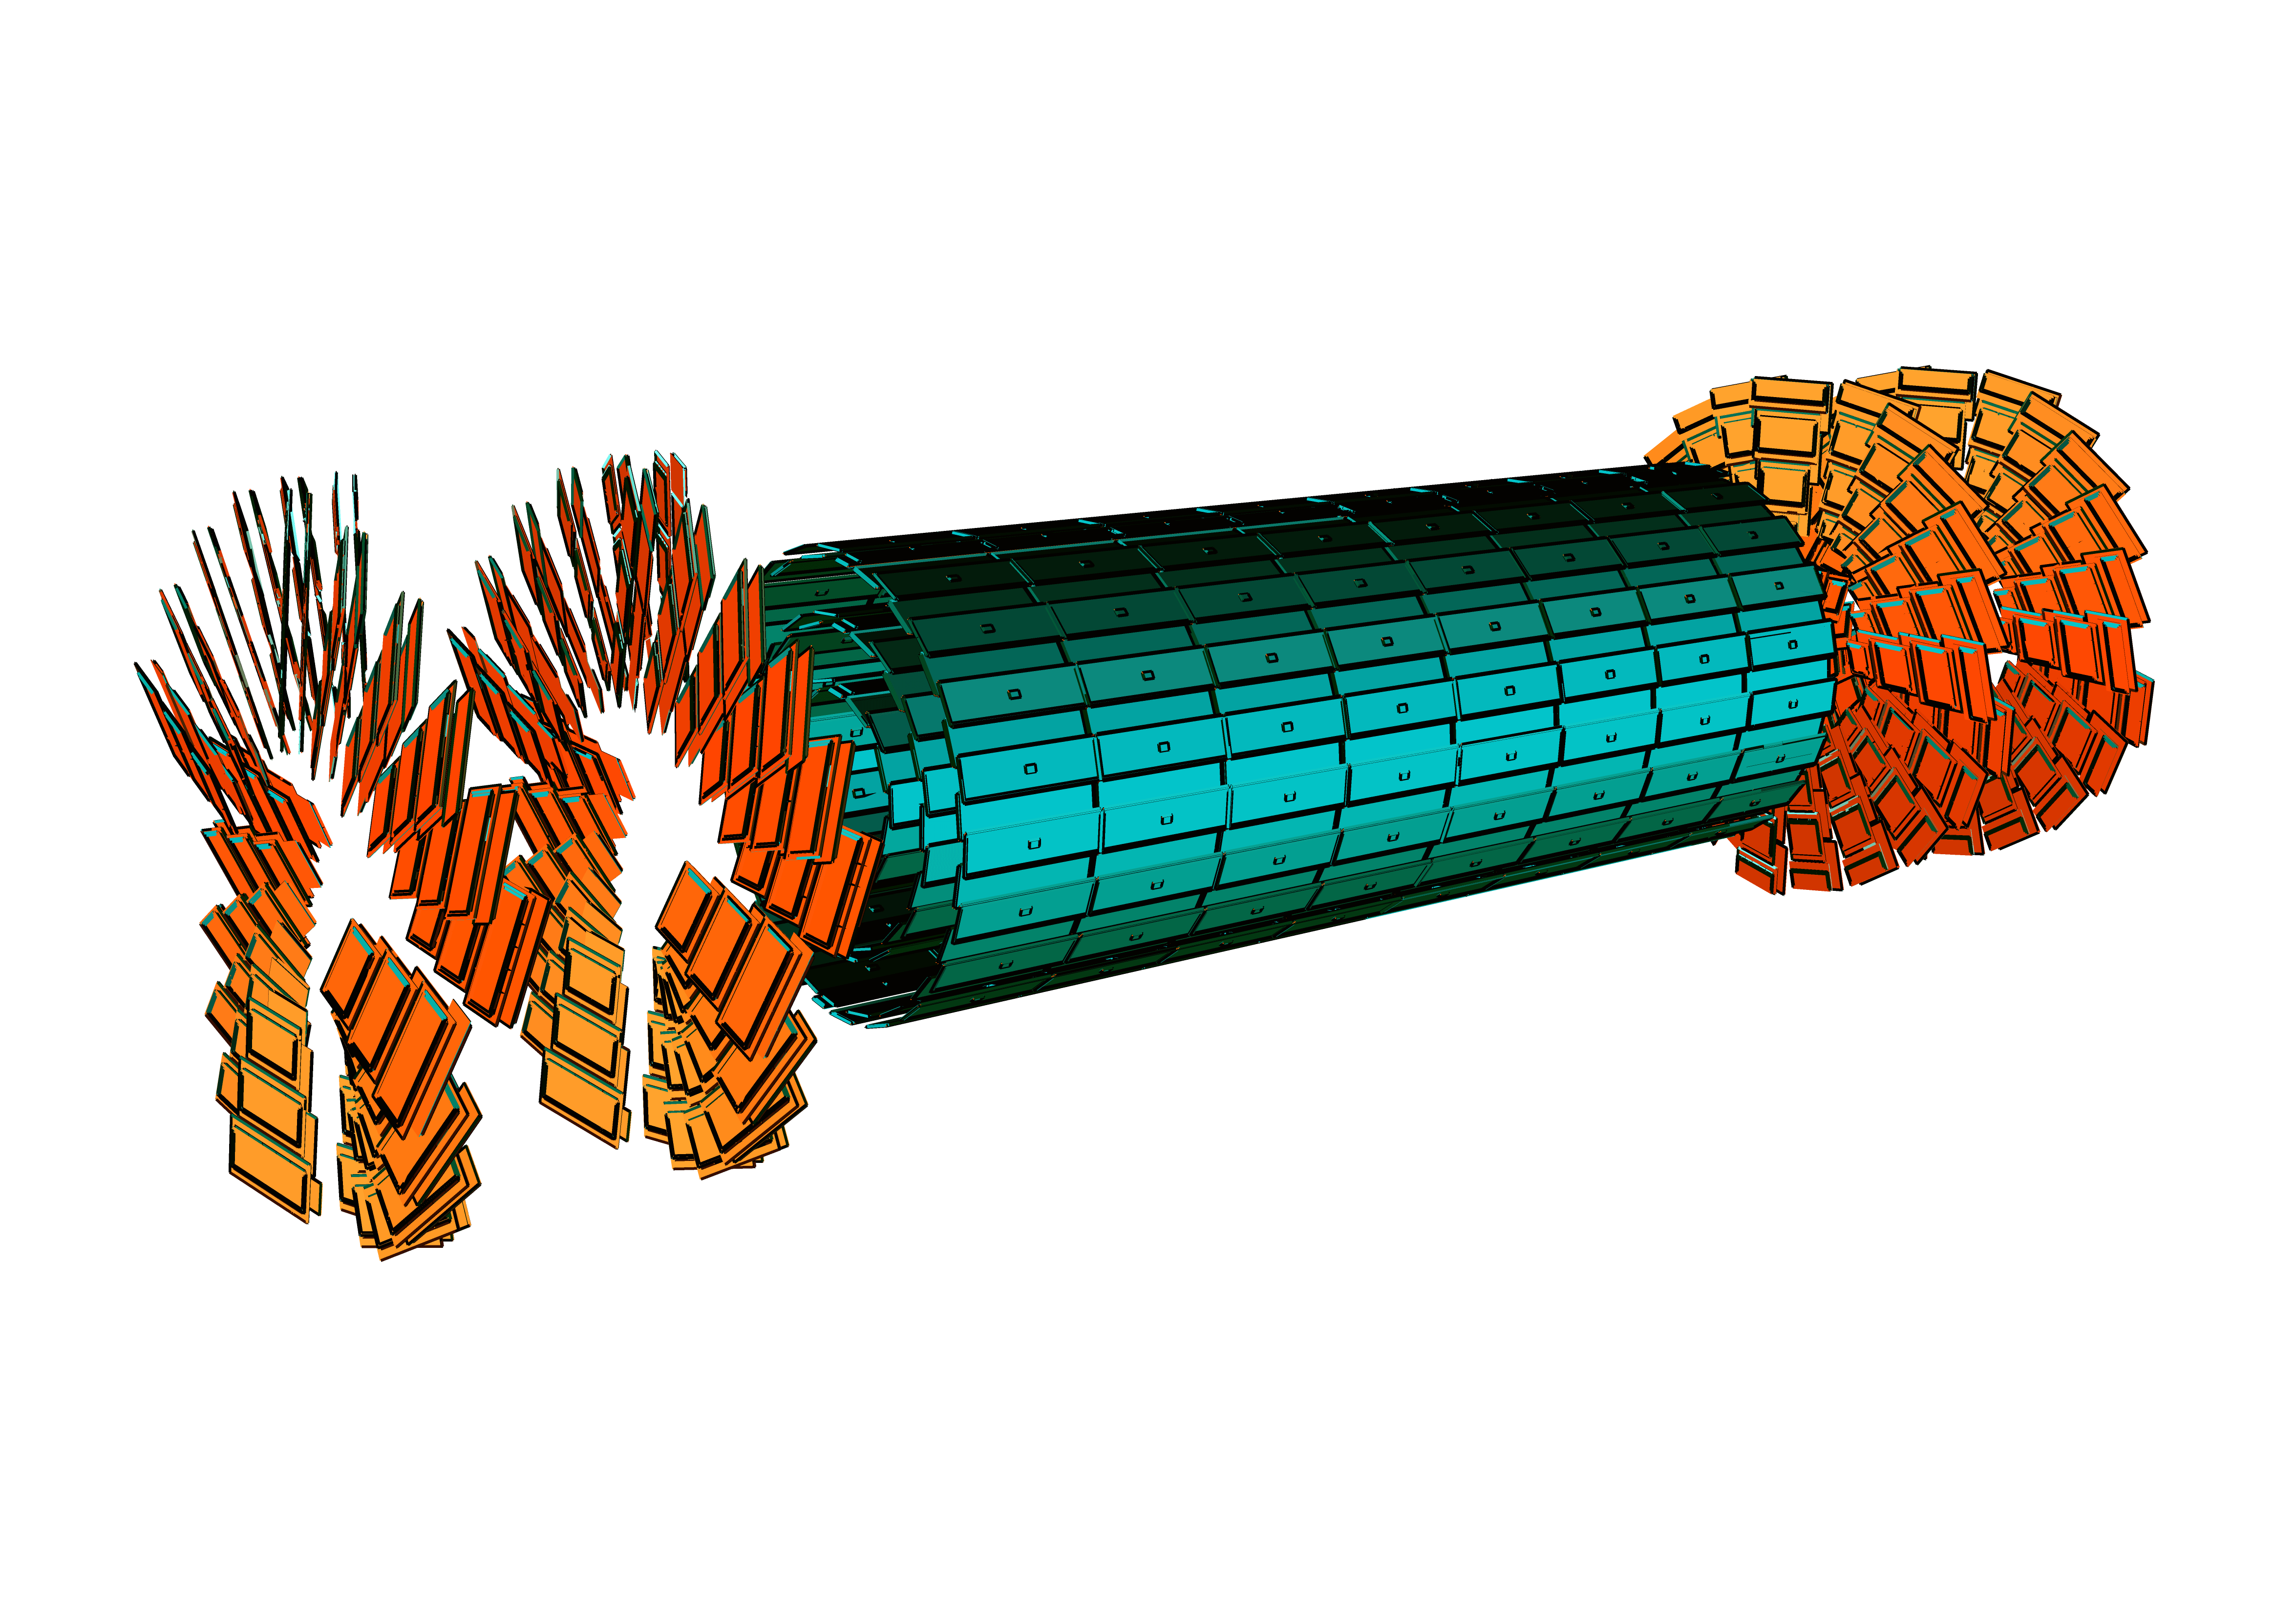
\includegraphics[width=.45\textwidth]{pics/pixel_diagram}
\end{center}
\caption{The CMS Pixel detector }
\label{fig:pixel}
\end{figure}

The CMS pixel detector (Figure \ref{fig:pixel}) consists of three layers are radii of 5.3 cm, 7.2 cm and 11 cm and 2 disks on each size of the barrel at 34.6 and 46.6 cm from the either side of the interaction point. 

\begin{figure}
\begin{center}
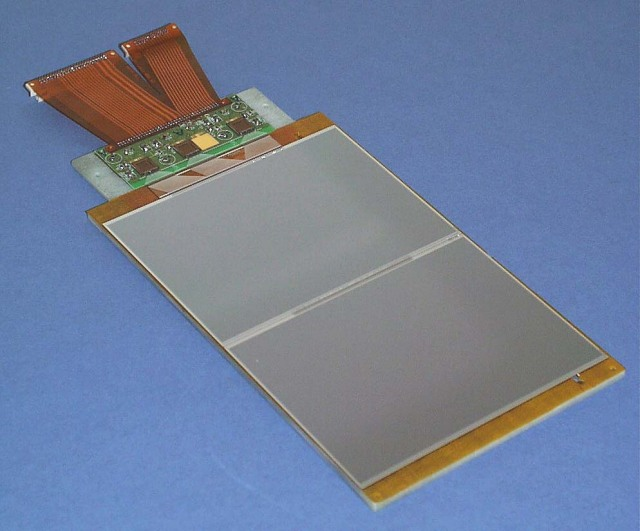
\includegraphics[width=.45\textwidth]{pics/tracker_module}
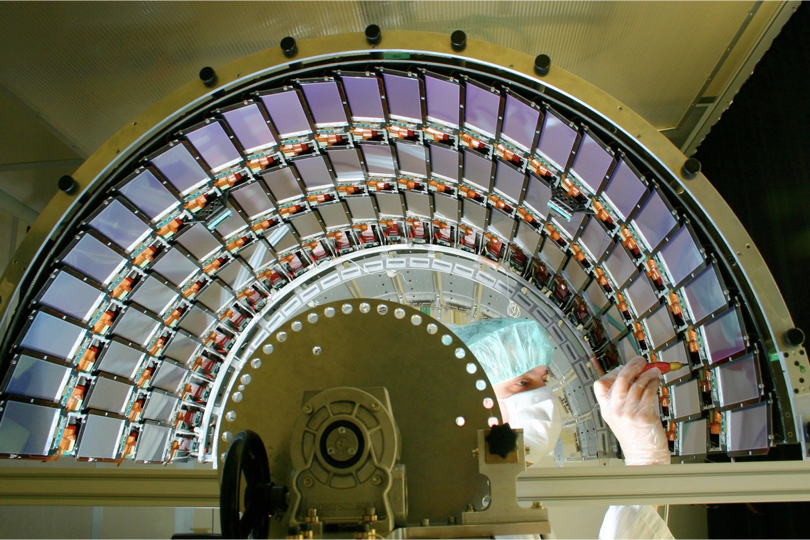
\includegraphics[width=.45\textwidth]{pics/tracker_strips}
\end{center}
\caption{A single CMS tracker module (left) and a tracker inner barrel module (right)}
\label{fig:tracker_strips_and_module}
\end{figure}

Track reconstruction is degraded by the interaction with the tracker material. With some finite probability
as a function of the material density and thickness, the track with randomly scatter. 

High energy charged particles for which the detector volume and strength of the magnetic field do not permit the track
to bend cause significant degregdation of momentum resolution as well as charge sign detrmination. For low energy tracks, 
the magnetic field 

\section{Muon Spectrometer}

\begin{figure}
\begin{center}
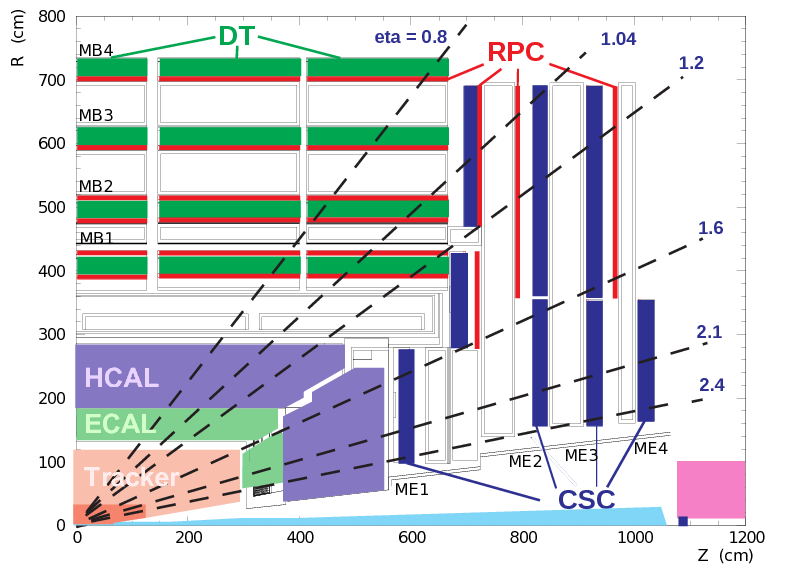
\includegraphics[width=.85\textwidth]{pics/muon_diagram}
\end{center}
\caption{Kinematic acceptance of the CMS Muon System}
\label{fig:muon_diagram}
\end{figure}

\begin{figure}
\begin{center}
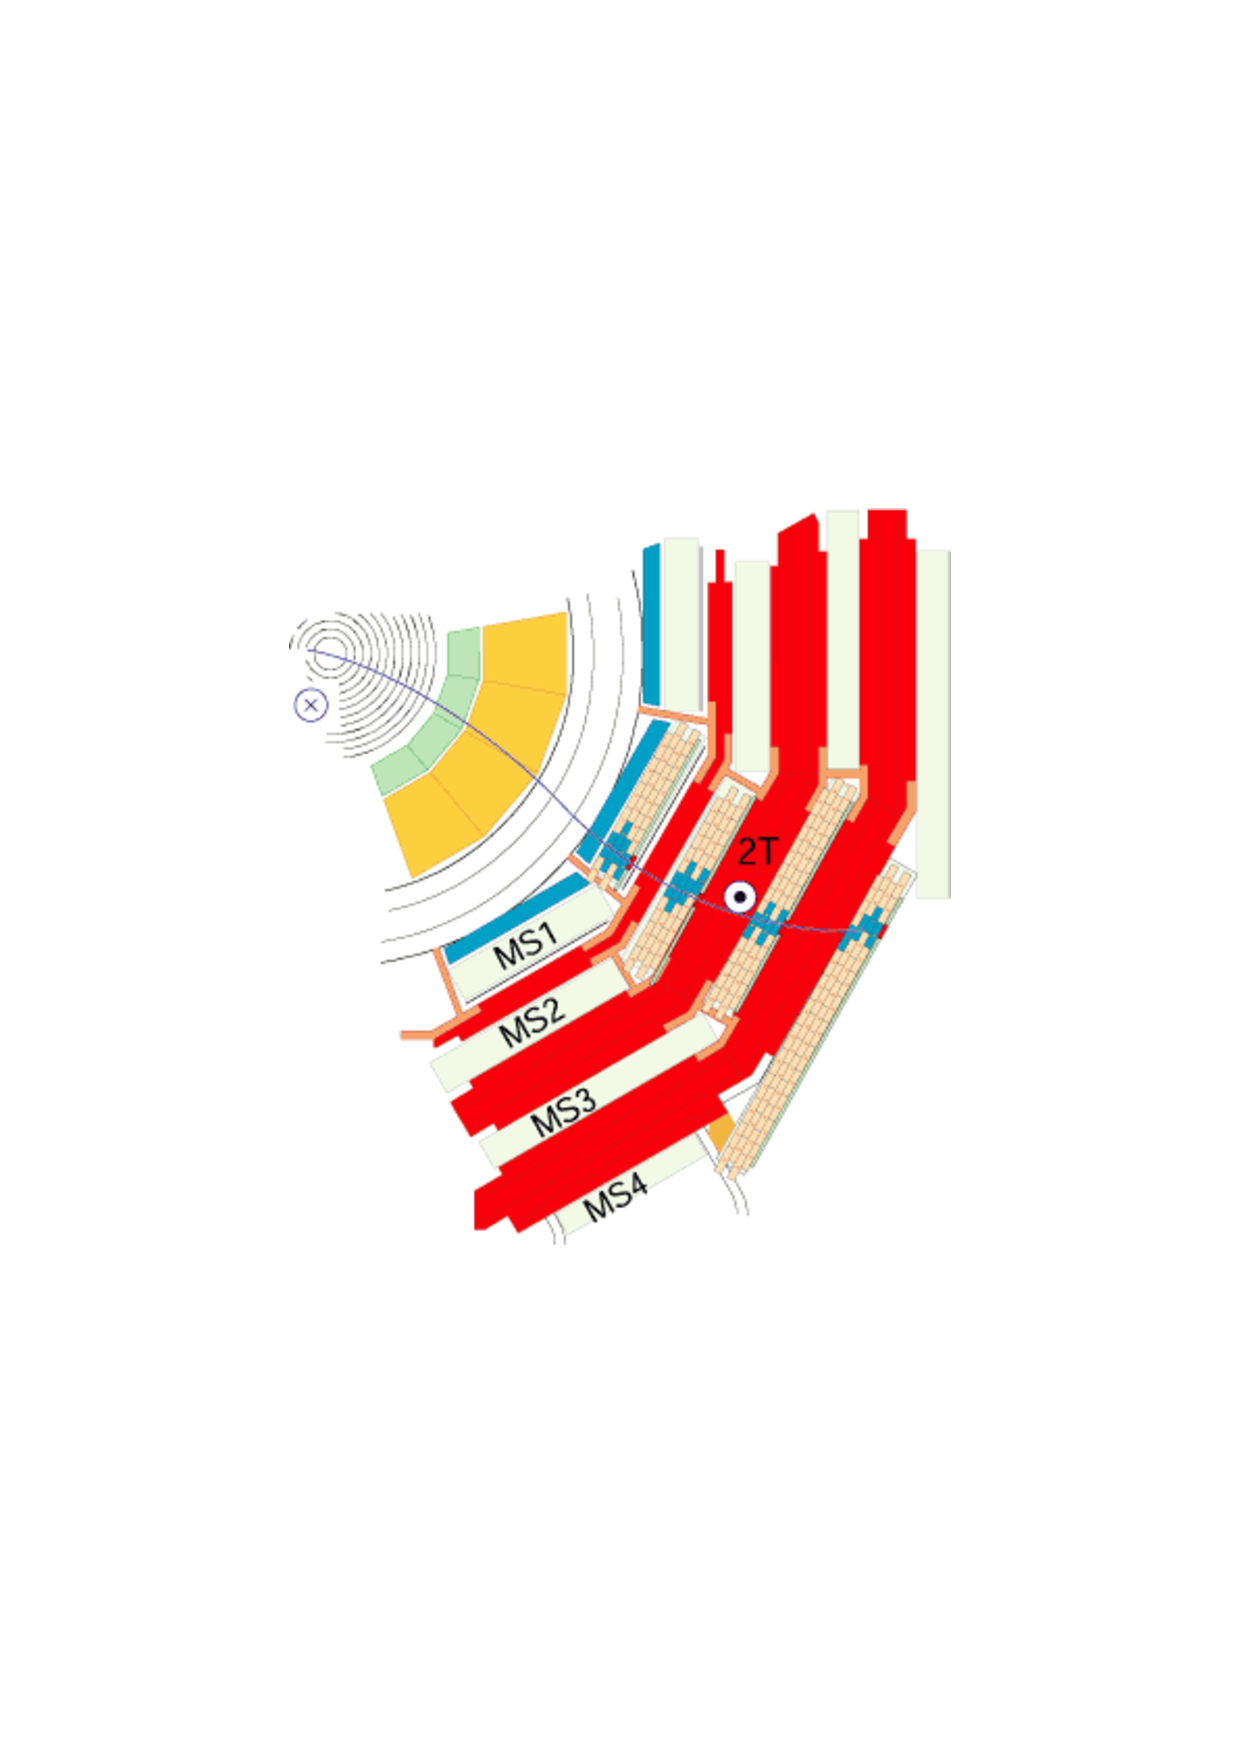
\includegraphics[width=.45\textwidth]{pics/muon_slice}
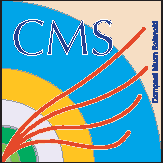
\includegraphics[width=.45\textwidth]{pics/cms_logo}
\end{center}
\caption{Slice of the muon detector (left) and cms logo (right)}
\label{fig:muon_slice}
\end{figure}


\begin{figure}
\begin{center}
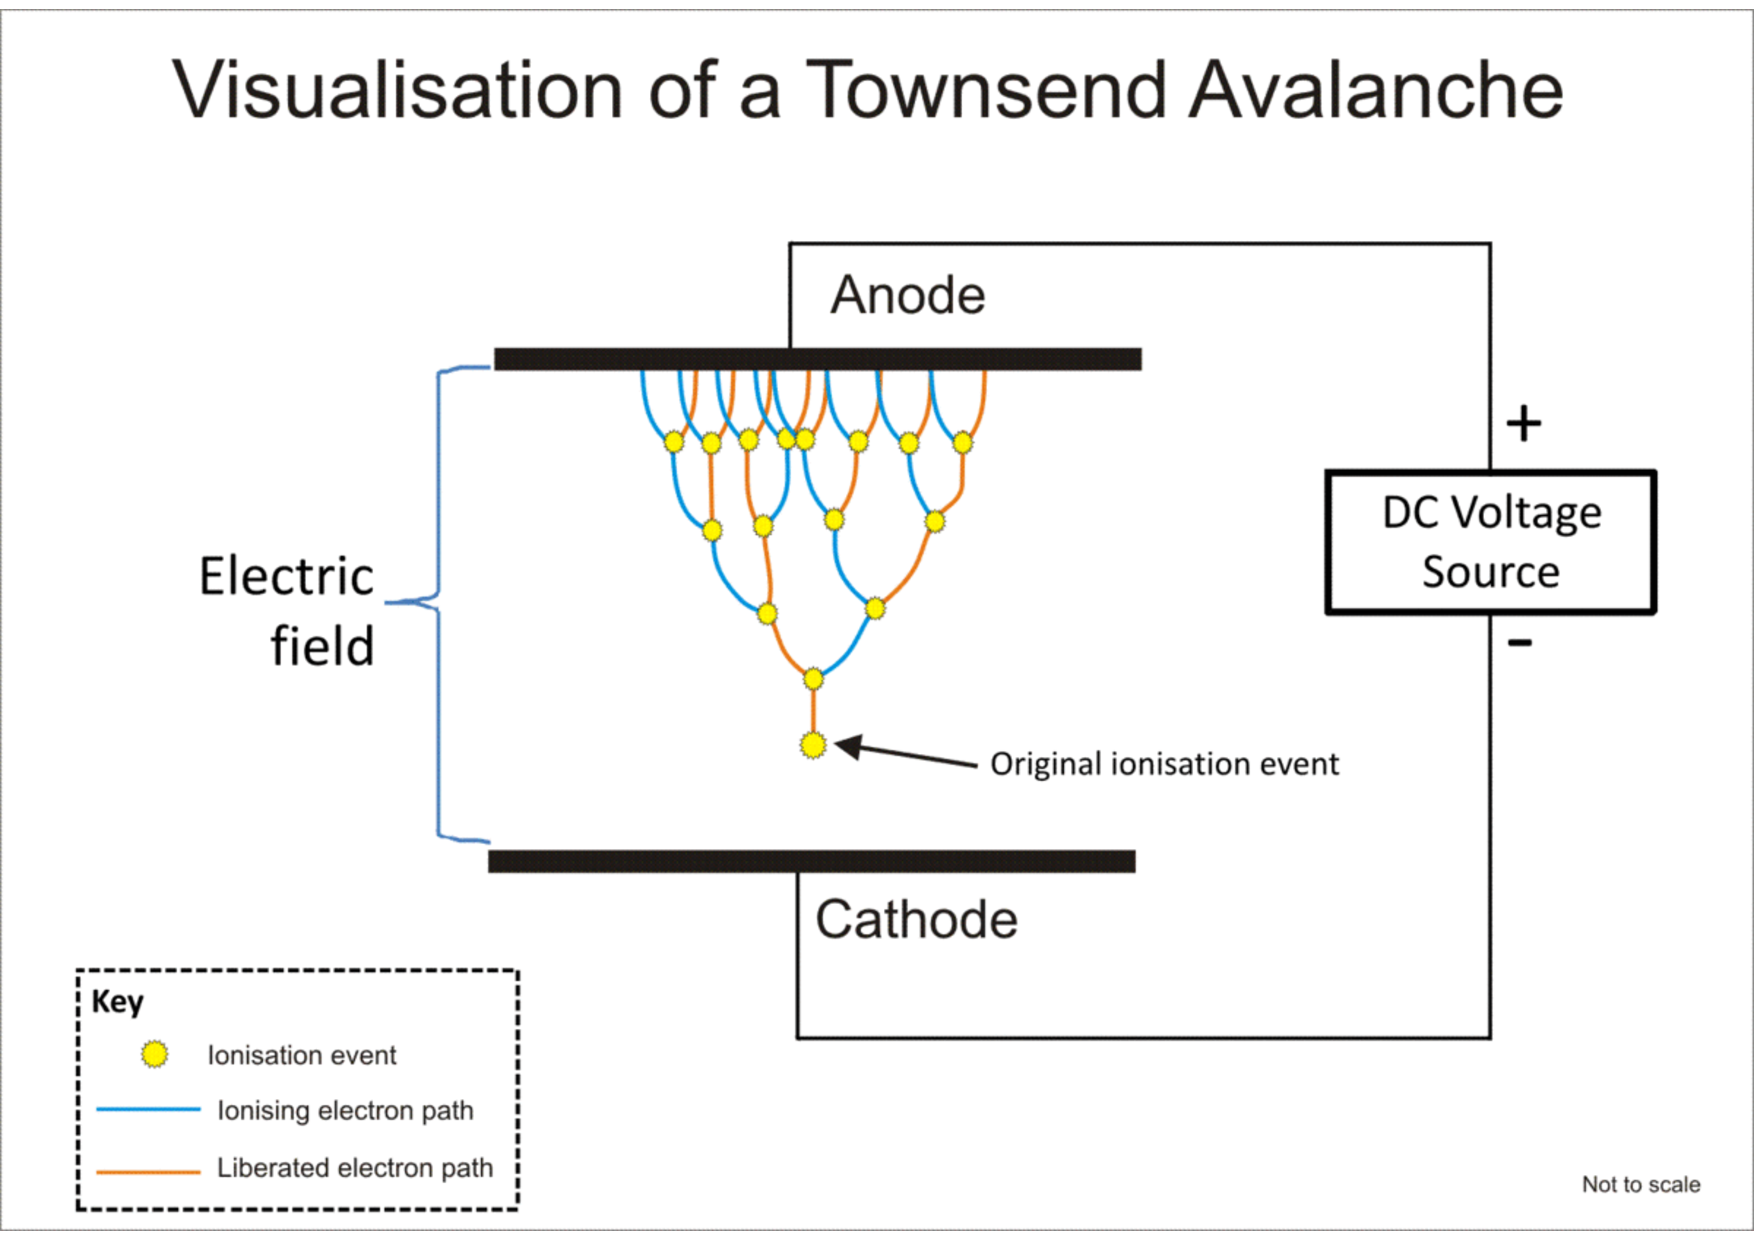
\includegraphics[width=.45\textwidth]{pics/avalanche}
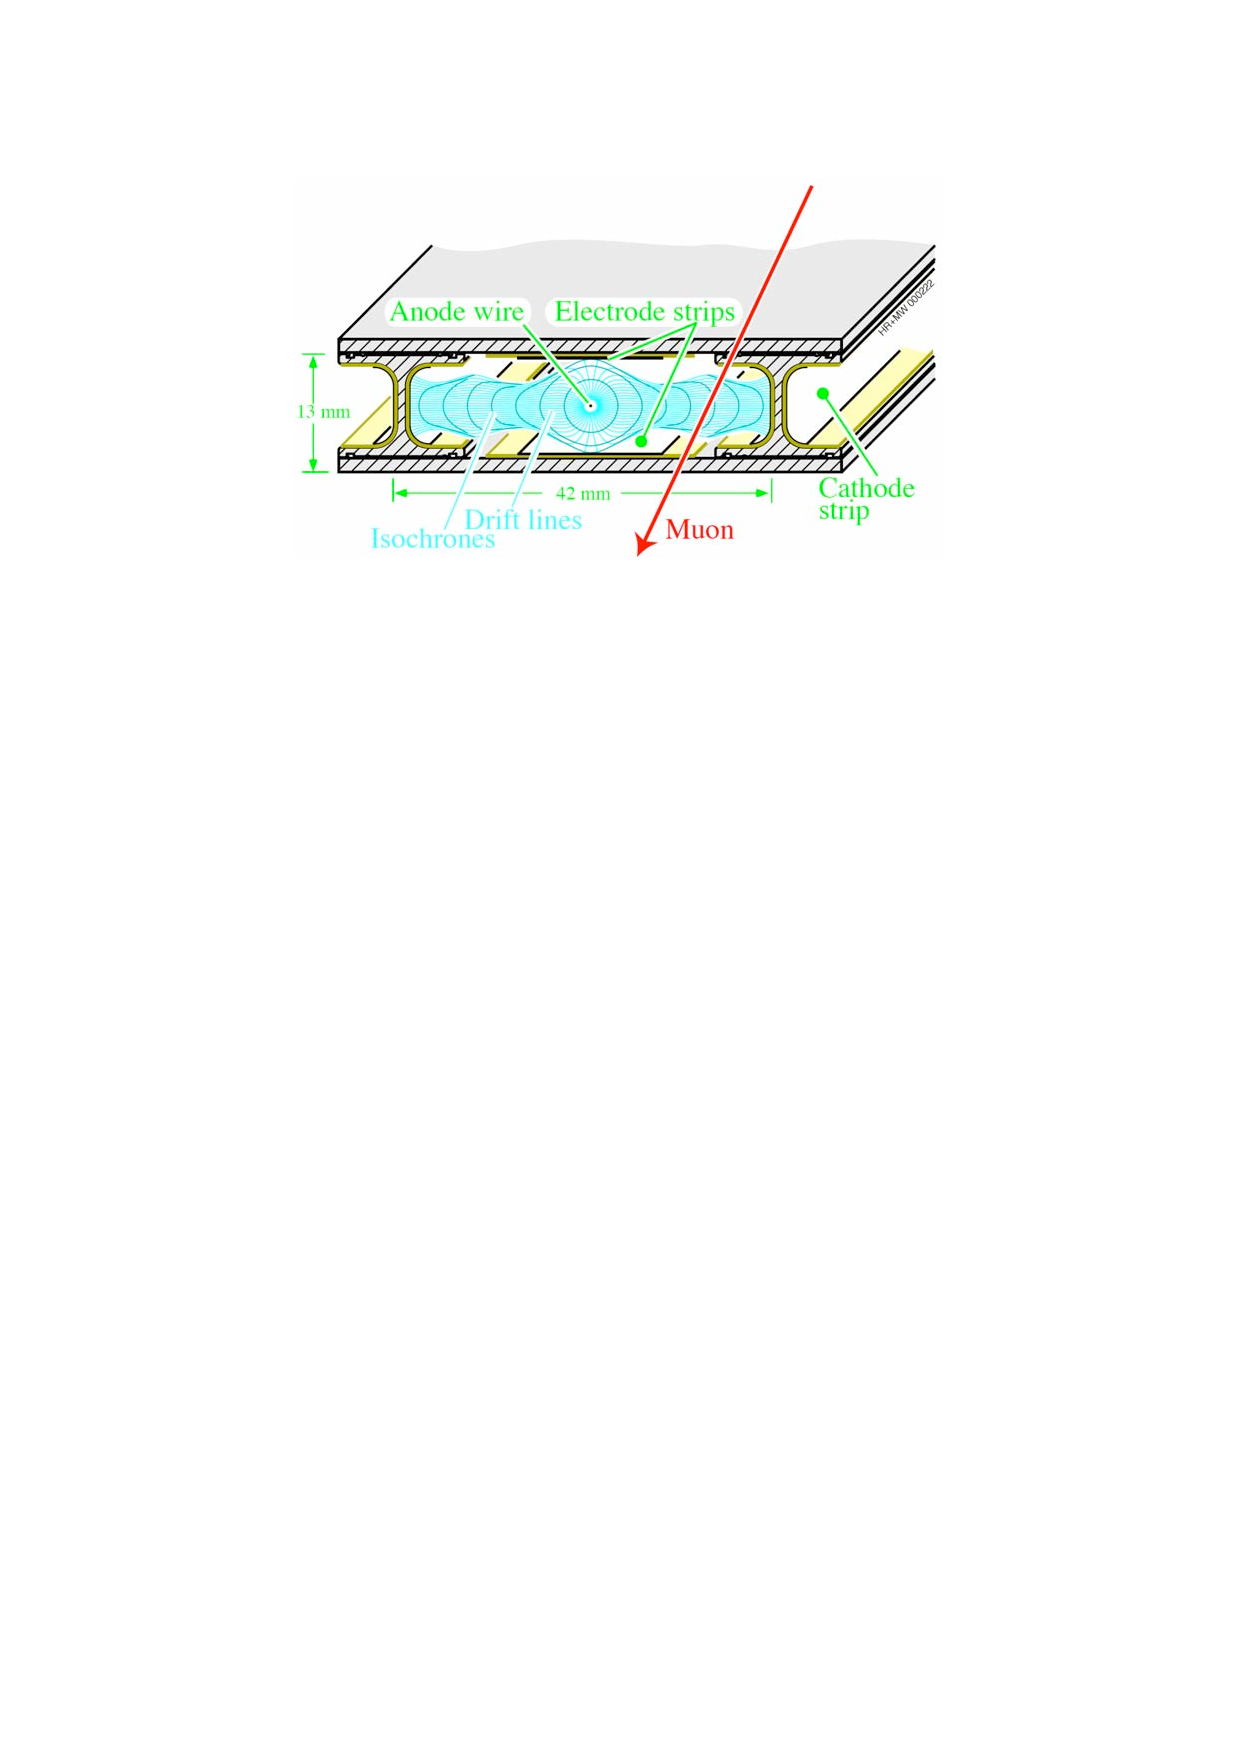
\includegraphics[width=.45\textwidth]{pics/cell_diagram}
\end{center}
\caption{When a gaseous medium is ionized by the track of a muon the resulting liberated electrons are accelerated
in the electric field and collide with gas molecules. The result is an avalanche of electrons collected at the anode. 
The processes is known as a Townsend Avalanche (left) The drift tube design showing the drift lines.  }
\label{fig:avalance}
\end{figure}

The Compact Muon Solenoid's name is partly taken from the Muon subsystem which is
 built to identify and measure the trajectories of muons. The search for displaced jets uses only calorimeter
quantities and inner tracking correspondingly no sensitivity to muons and no muon vetos.
 This section is included only for completeness.  

The muon system consists of 3 separate detectors: drift tubes (DT's), resistive plate chambers (RPCs), and 
cathode strip chambers (CSCs). All three systems rely on the ionization of a gas medium caused by the charged muon's
traversal through the detector. The detectors are multi-layered and sandwiched betwen between layers of the iron  return
yoke (Figure \ref{fig:muon_diagram}). The iron layers aid in particle identification by stopping nearlly all
 other particle activity before the final detector layer. As  muons are very weakly interacting, they should be the only
particles reaching the edge of the detector. When the magnetic field changes outside of the solenoid, muon tracks
will change curvature in the muon system as depicted in the CMS logo (Figure \ref{fig:muon_slice}). The second measurement
made in the muon spectrometer improves the momentum resolution for energetic muons $>100 GeV$, however lower momentum muons are dominanted by a increase of multiple scattering from the additional detector material. 

It the context of long-lived searches it is interesting that the muon is the only long-lived fundamental particle, with
 a finite lifetime of $\tau_0=2.2 \mu$s or equivalently $c\tau_0 = $ 660m. The dominant decay to an electron and two neutrinos  is suppressed by requiring the muon decay with an  offshell decay through the much heavier $W$. 
This method of generating long-lived signatures mirrors the motivations of
split supersymmetry where the gluinos are long-lived as they must decay through much heavier squarks.
If this were the end of the story we would expect $\approx$ 1\% of muon decays to occur before the final layer.  However, a moderately energetic muon will experience time dilation $c\gamma\tau_0$ in the lab frame with 
$\gamma = E / m = (1$ GeV$)/ 105$ MeV $\approx 10$. Accordingly, on detector length scales $O(10$ m$)$ energetic muons can be considered stable. 

The drift tube system located in the barrel region covers $|\eta| < 1.2$ with 4 concentric rings (segmented in $r=4.0,4.9,5.9,7.0$ m) referred to as ``stations''. Five divisions are also made in 
the $z$ direction referred to as ``wheels'' partitioned into 12 sectors of 30 degrees.  The three inner cylinders have 
60 chambers each and the outer cylinder has 70.   Each chamber measures 3.0m x 2.5m.
 Each chamber is divided into 3 (or 2) super layers with 4 drift cells per layer (2 in $\phi$, 2 in $z$). The drift cells
use  anode wires at voltage of $+3.6$ kV, electrode strips at 1.8kV and -1.2kV cathode strips  to detect the localized ionization showers from muon tracks (Figure \ref{fig:avalanche}). The full system includes 172,000 wires.  The maximal path of drift is 21 mm corresponding 
to a drift time of 380ns in a gas mixture of 85\% Argon and 15 \% CO$_2$. (cite-complete-cms-description)

The CSCs and DTs are  located in the endcap region. The CSCs are located between $0.9 < |\eta| < 2.4$ and the RPCs between $0.9 < |\eta| < 1.6$. There are 4 stations for each endcap. The CSCs are trapezoidal multiwire proportional chambers comprised
 of 6 wire planes interleaved with 7 cathode panels. The chambers extend 1.7 (or 3.4) m 
in the radial direction covering 10 or 20 degrees. Each chamber layer 
Wires running in the $\phi$ direction define a tracks radial position. The $\phi$ 
coordinate along the wires is obtained by interpolating charges induced 
on the cathode strips. 


\begin{figure}
\begin{center}
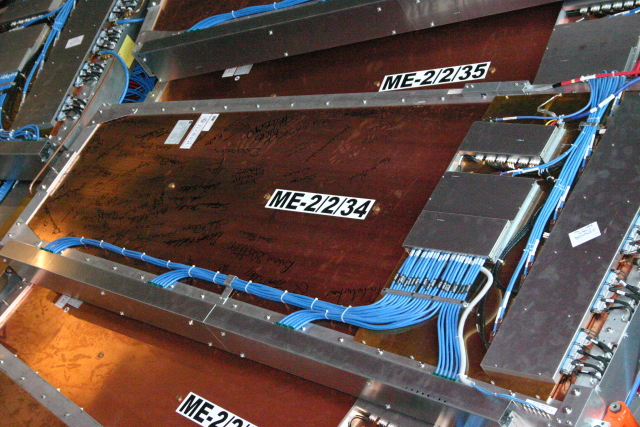
\includegraphics[width=.45\textwidth]{pics/cathode_strip_chamber}
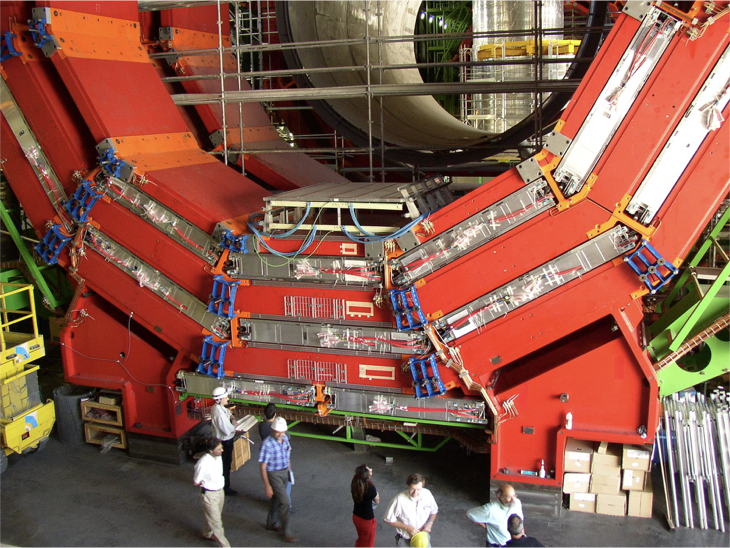
\includegraphics[width=.45\textwidth]{pics/rpc_plates}
\end{center}
\caption{The Muon Cathode Strip Chamber}
\label{fig:strip_chamber}
\end{figure}


\section{Trigger System}

\begin{figure}
\begin{center}
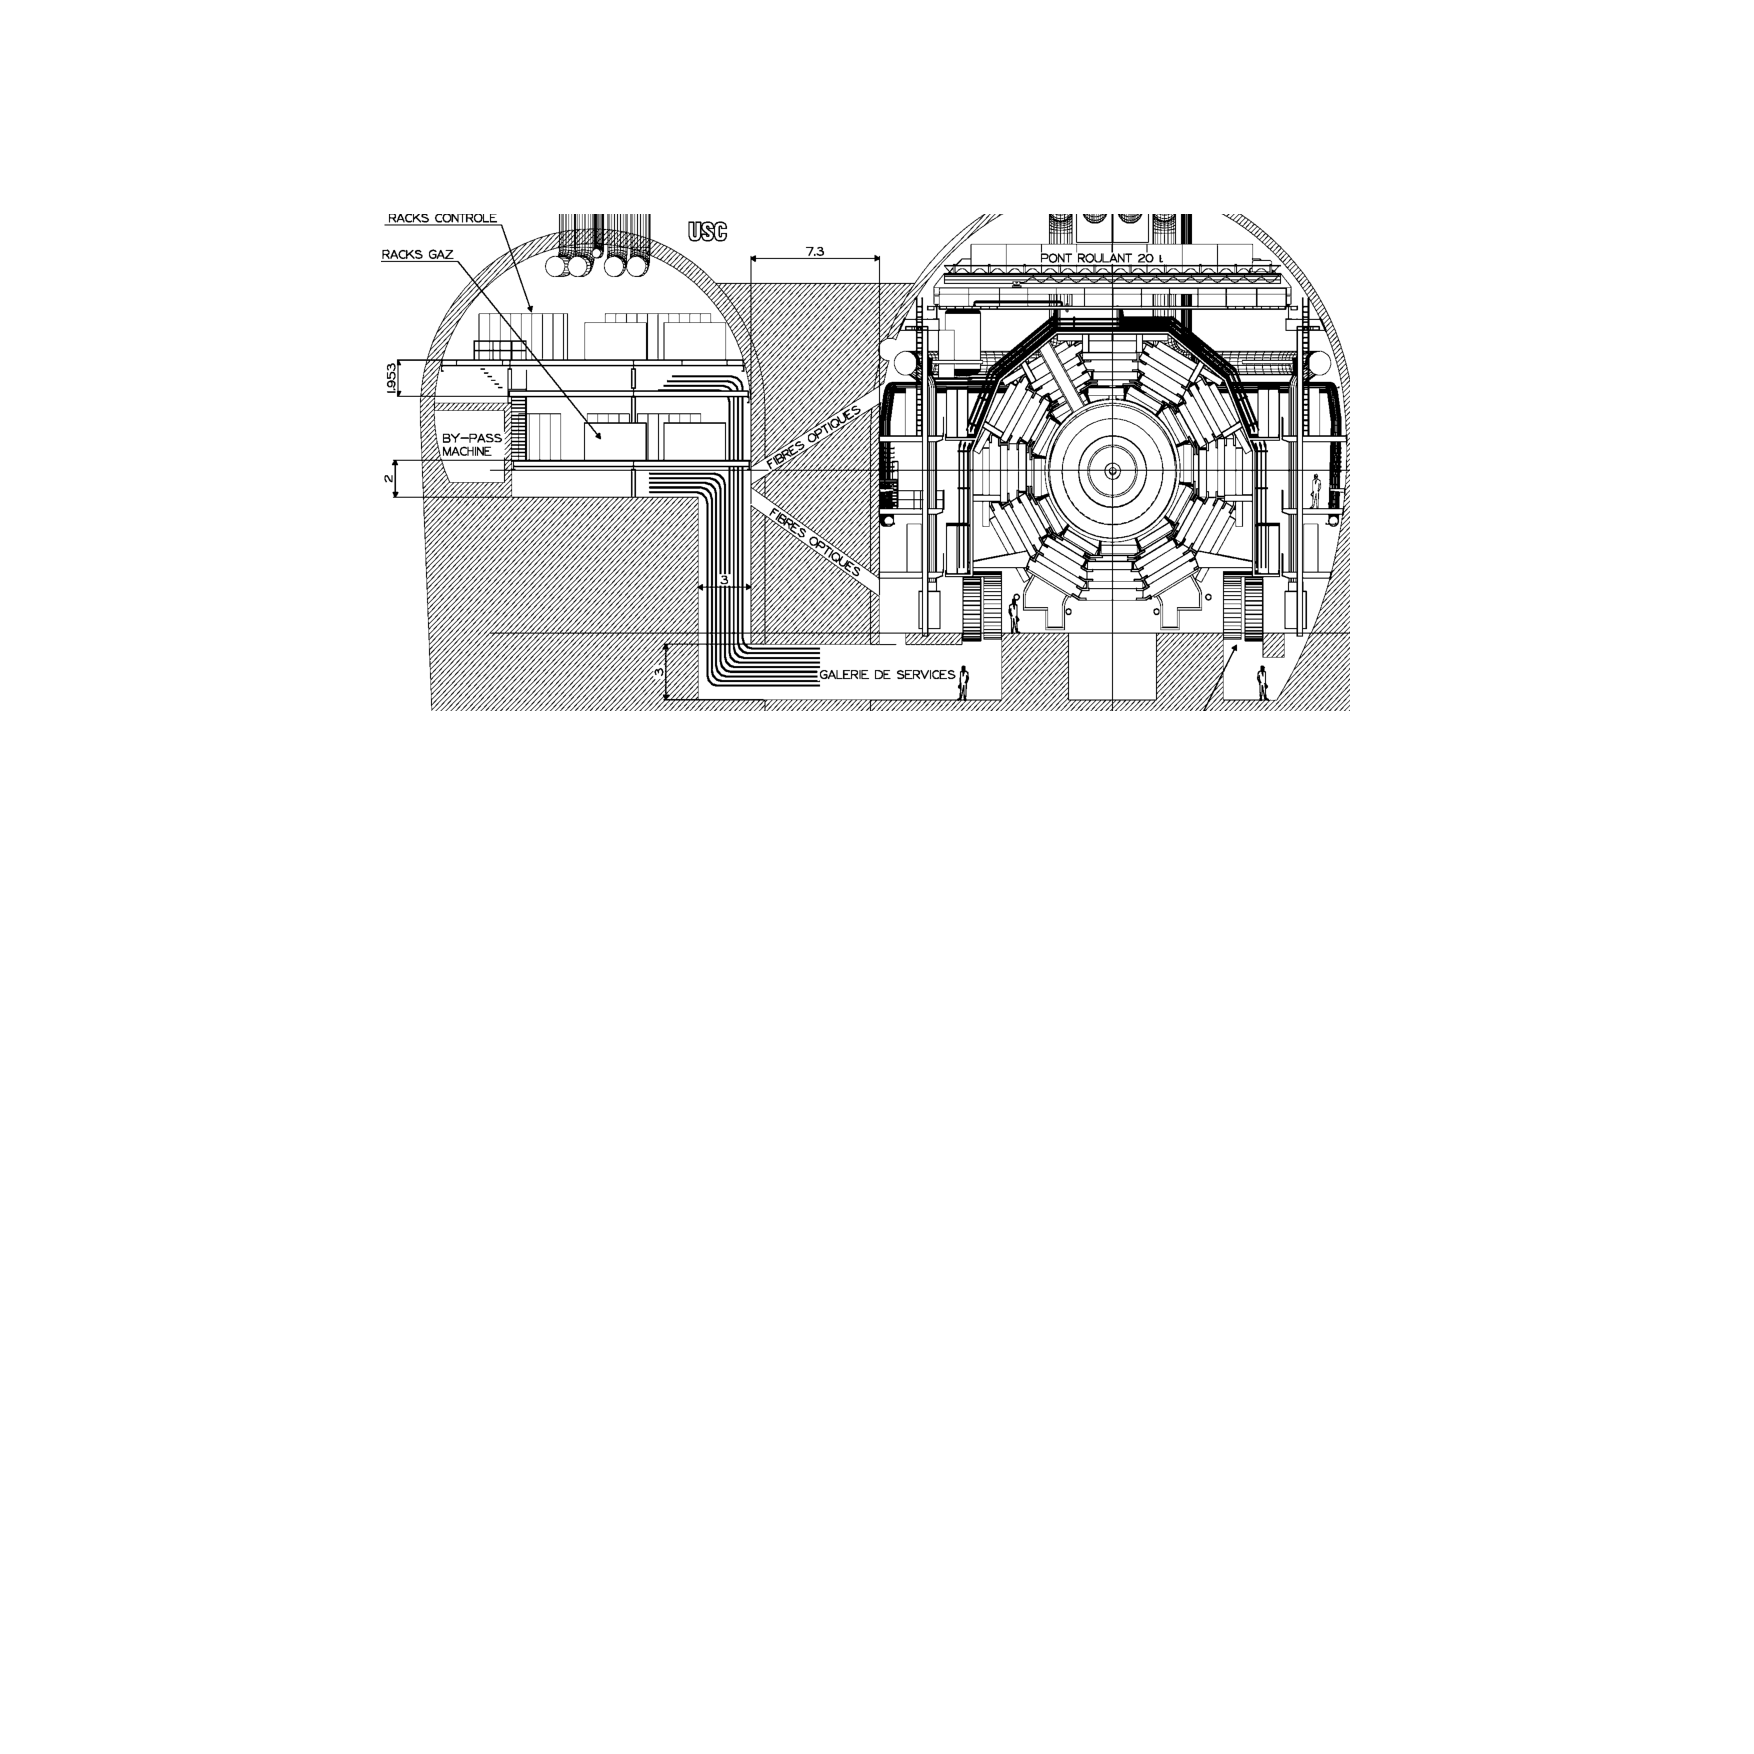
\includegraphics[width=.95\textwidth]{pics/counting_room}
\caption{Location of the counting room relative to the experimental hall}
\end{center}
\label{fig:counting_room}
\end{figure}

\begin{figure}
\begin{center}
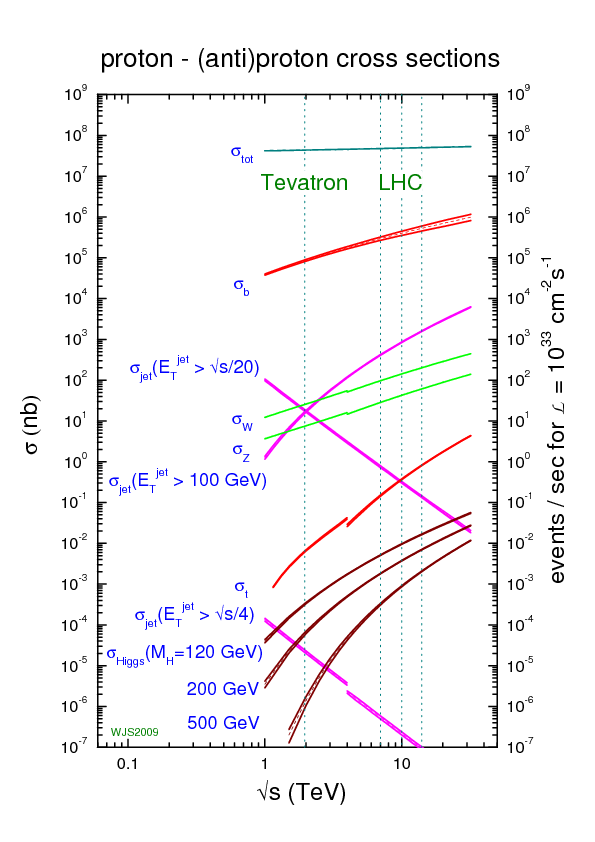
\includegraphics[width=.5\textwidth]{figures/exp_proj/pdf_xsec.png}
\caption{Common cross sections of proton collisions as a function of the center of mass energy $\sqrt{s}$}
\end{center}
\label{fig:pdf_xsec}
\end{figure}

The CMS Trigger System exists as a filter through which events are determined to be interesting or 
useful enough to be written down. The name comes from the nature of algorithms used to determine 
what to write down. If an event passes any of the online algorithms, this ``triggers'' the collision to be 
written down in its entirety regardless of the goals of the path in particular 
 (albiet with some notable exceptions). It is both  unnecessary and impractical to record every
collision the LHC delivers. The low momentum transfser  hadronic events contained in the vast majority of
 proton collisions is well understood from past experiments. Figure \ref{fig:pdf_xsec}  shows 
typical physics processes for proton-proton scattering. Events such as the production 
of a $b$ quark  occur at $\approx 10^6$ Hz at a luminosity of $\mathcal{L} = 10^{33}$ cm$^{-2}$ 
whereas processes of interset, such as the production of the Higgs is much lower at $\approx 10^{-2}$ Hz.  

The LHC has beam crossings at a rate of $\approx 40$ MHz with 
each crossing coming spaced at $\approx$ 25 ns. The number of ineleastic collisions per bunch cross crossing
 is given by the  is the total inelastic cross section times the luminosity divided by the bunch collsion rate. 
This is respectively $8.5\times 10^{-26}\text{cm}^2 \times 10^{34}\text{cm}^{-2}\text{s}^{-1}/ (40 \times 10^6 \text{s}^{-1} \approx 24$ (cite:arXiv:1204.5689). 
The collisions are stored with an average file size 1 MB in their unprocessed form in a format refered to as \texttt{RAW}. However the bandwidth for the combined constraints of
 aquisition rate, storage and processing, is limited to $10^3$ Hz and equivalently $10^3$ MB/s. 
Generally, all but one of the inelastic collisions is interesting and a large excess of  
activity is generated in the detector electronics. The trigger must be robust enough to select 
these events efficiently while remaining  efficient in maximizing the limited bandwidth.  

\begin{figure}
\begin{center}
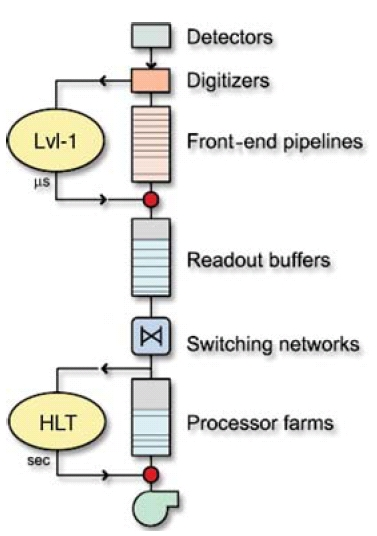
\includegraphics[width=.4\textwidth]{figures/exp_proj/cms-trigger}\\
\caption{A diagrammatic representation of the level 1 and HLT trigger processing (cite-tridas-tdr)}
\label{fig:l1_hlt_diagram}
\end{center}
\end{figure}

The CMS Trigger system is designed to read events at the event crossing frequency and generate the
 factor $10^5$ of rejection between the crossing frequency and the archival capacity. This factor 
is too large to achieve in a single step given the complexity of triggers and event reconstruction necessary
to build efficient algorithms. Therefore the task is split into two steps The Level 1 (L1) and High Level
 (HLT) Trigger systems (Figure \ref{fig:l1_hlt_diagram}). The L1 system is a coarse study of an event designed
 to be fast and capable of analyzing every event at 40 MHz. The HLT provides the flexibility the L1 lacks 
permitting as much event reconstruction 

%% The $O(10^7$) events per second first pass through the L1 Trigger which reads out events at $10^5$ Hz. 
%% From here, the High Level Trigger makes the final decision as to which events are kept. 
%% Approximately 350 Hz is processed and stored, 300 Hz is ``parked'' (stored but processed later), 
%% and 1 kHz is partially stored (only the HLT level information and not the RAW detector information) 
%% and used for data scouting for future analysis.  

The most obvious criterion for interesting events are hard physics events with high momentum transfer, $q^2$, and
correspondingly large transverse momentum.
 As the protons collide with effectively no transverse momentum, any event with significant deposits of 
transverse energy (or even missing transverse momentum) is indicative of a hard physics process. 
The total transverse energy of an event falls off exponentially, so a simple way to
reduce the rate of processed events is to raise the energy requirements of accepted events. However,
given the increasing luminosity of the LHC the thresholds are encroaching upon Standard Model physics processes
like single $W$ production where triggering on every single-electron event is a reaching kinematically limited regime. 

The particulars of a given high level trigger path is dictated by their use case. Generally, analyses 
searching for new physics are categorized by their final state signature. Correspondingly,
 the trigger requires loose identification 
on the objects of that signature such as the isolation and shape of energy deposition.  Additional,
global requirements such as angular separation, or the invariant mass of two objects is common as well.
Once the event has passed the Level 1 and HLT Triggers, tighter and more computationally 
costly selection can be made offline where we are unrestricted by bandwidth limitations. 

\subsection{Level 1 (L1) Trigger}

The L1 Trigger is built using custom hardware composed of field programmable gate arrays (FPGAs), 
application-specific integrated circuits (ASICs) and programmable look up tables (LUTs). 

The Trigger Primitive Generators (TPGs) are locally constructed from the energy deposits in the calorimeters or
hits/track-sgements in the muon chambers. The regional reconstruction applies coarse pattern
 recognition to the primitives and combines them. Together the  Global Calorimeter Trigger (GCT)
 and Global Muon Trigger (GMT) are processed at the global trigger (GT) to decide whether or
 not an event is kept. It is important to note that there is no inner tracking performed at this
 level (only muon specific tracking). Track building is time intensive and cannot, in its current
 state, be performed reliably at speeds comparable to the bunch crossing frequency. 
Future upgrades are planned to include tracking at the L1 which would significantly aide in
 the detection of soft hadronic signatures with specific track toplogies (ex. displaced signatures and VBF SM Higgs Production in decays to $b\bar{b}$). 

\begin{figure}
\begin{center}
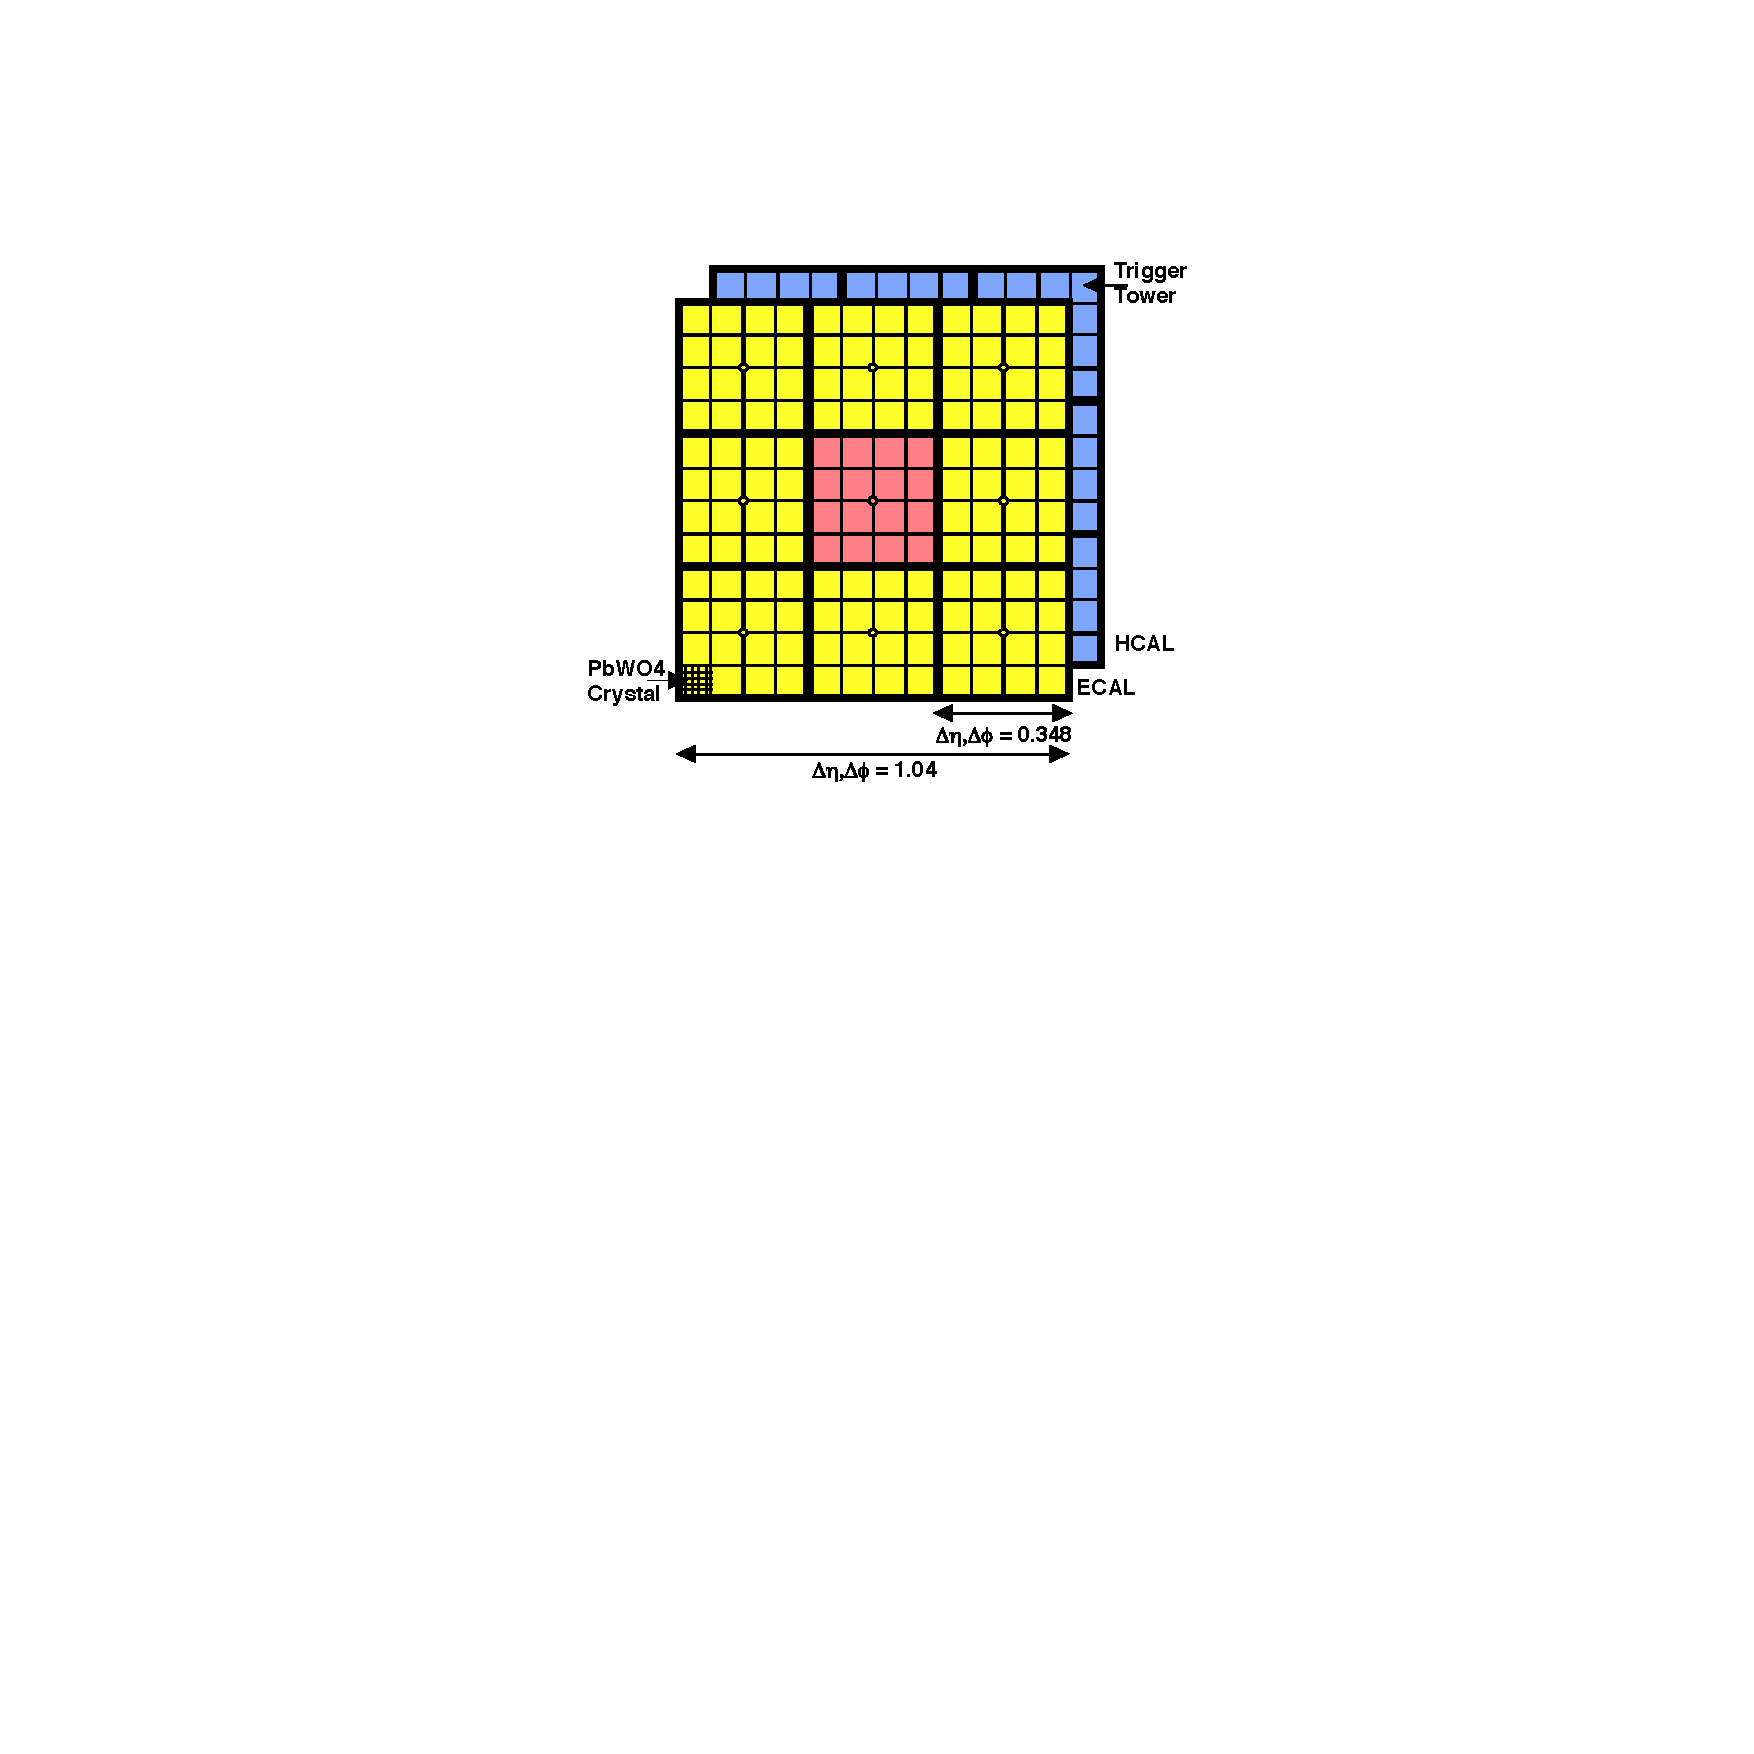
\includegraphics[width=.55\textwidth]{pics/jet_trigger_tower}
\caption{A  representation of a jet as assembled from the ECAL and HCAL trigger primitives. (cite-tridas-tdr)}
\end{center}
\label{fig:jet_trigger_tower}
\end{figure}

The jet trigger primitives are built from transverse regions of 12 x 12 grids constructed from 

The regional calorimeter trigger (RCT) collects regional transverse energy sums segemented in variable size
 trigger tower arrays summed between the ECAL and transverely adjacent HCAL within $|\eta| < 5.0$. Electrons
and photons use the same size 

\subsection{High Level Trigger (HLT)}

\begin{center}
\begin{table}[]
\begin{center}
\caption{High Level Trigger filter farm configuration in 2015 \cite{timing}}
\begin{tabular}{cccc}
Install Year: & 2011 & 2012 & 2015 \\  
\hline
CPU & X5650  & E6-2670  & E6-2680v3  \\
Architecture & Westmere  & Sandy Bridge & Haswell \\
CPUs per board & 2 & 2 & 2 \\
Cores/CPU & 6 & 8 & 12 \\
RAM & 24 GB & 32 GB & 64 GB \\
Clock Rate (w/Boost) & 2.66 (3.06) GHz & 2.60 (3.30) GHz & 2.50 (3.30) GHz \\

Total Cores (Boards) & 3456 (288) & 4096 (256) & 8640 (360) \\ 
\end{tabular}
\end{center}
\end{table}
\end{center}


Algorithms at trigger stage are referred to as paths. The entire collection of paths is referred to
 as a trigger menu. As the physics goals of the experiment change and machine luminosity ramps, 
the menu must evolve and adjust the thresholds within a given menu. The HLT is a crucial component of CMS data taking, as new physics that is never written down is never discovered. Problems with the offline
 reconstruction can be fixed at a later date by reprocessing the RAW data, but problems with the online reconstruction as performed by
the trigger paths) is permanent in the data collected. 

The paths are configured as a series of re-usable modules that either build an object (producers) 
or terminate the execution of the path based on some quantity (filters). The paradigmn ensures, that a producer which creates, say, the sum of transverse energy in the detector, is processed exactly once, despite being used by multiple paths. Ensuring that modules are reusable and reused greatly minimizes timing overhead of additional
paths. Common sequences, such as unpacking the calorimeter energy, are utilized by nearly every trigger. CMS as an experiment excells from a monolithic approach to its sofwatre where, the same software (known as CMSSW) is
 for analysis and data processing is used online.

The development, debugging, and testing of these menus
is a large organizational effort that requires the input from nearly every level of the experiment. 
Physics Object Groups (POGs)  e/gamma, Muons, Jets, and B physics must build
the online reccomendations for object identification and ensure their the performance with the varied 
paths which use them. Physics Groups (Higgs, Exotica, SUSY, ect.) must develop paths and justify the
added physics value of the individual paths in terms of their sensitivity. The Detector Performance Groups (DPGs) must provide object energy calibrations for the online energy reconstruction which differs significantly from
the offline reconstruction. 

Additionally, the DPGs must implement separate data streams, which save a much
smaller event content, to calibrate the detector. For instance a separate data stream exists for collecting
the copious production of $\pi^0$ and $\eta^0$ mesons which predominantly decay to two photons. The stream 
performs only the reconstruction of the ECAL and searches for low $p_t$ clusters within an invariant mass window.Saving only the hits corrsponding to these clusters reduces the event size from 1 MB to 2kB allowing the stream
to aquire events at a rate of 7kHz while maintaining a small bandwidth. For comparison, the physics data 
stream writes at 1000 Hz. 

The CMS HLT System is built from a varied collection of commercially available CPUs  comprising more than 16,000 cores in 2015 (Table \ref{tab:daq_diagram}). 


\subsection{DAQ}

\begin{figure}
\begin{center}
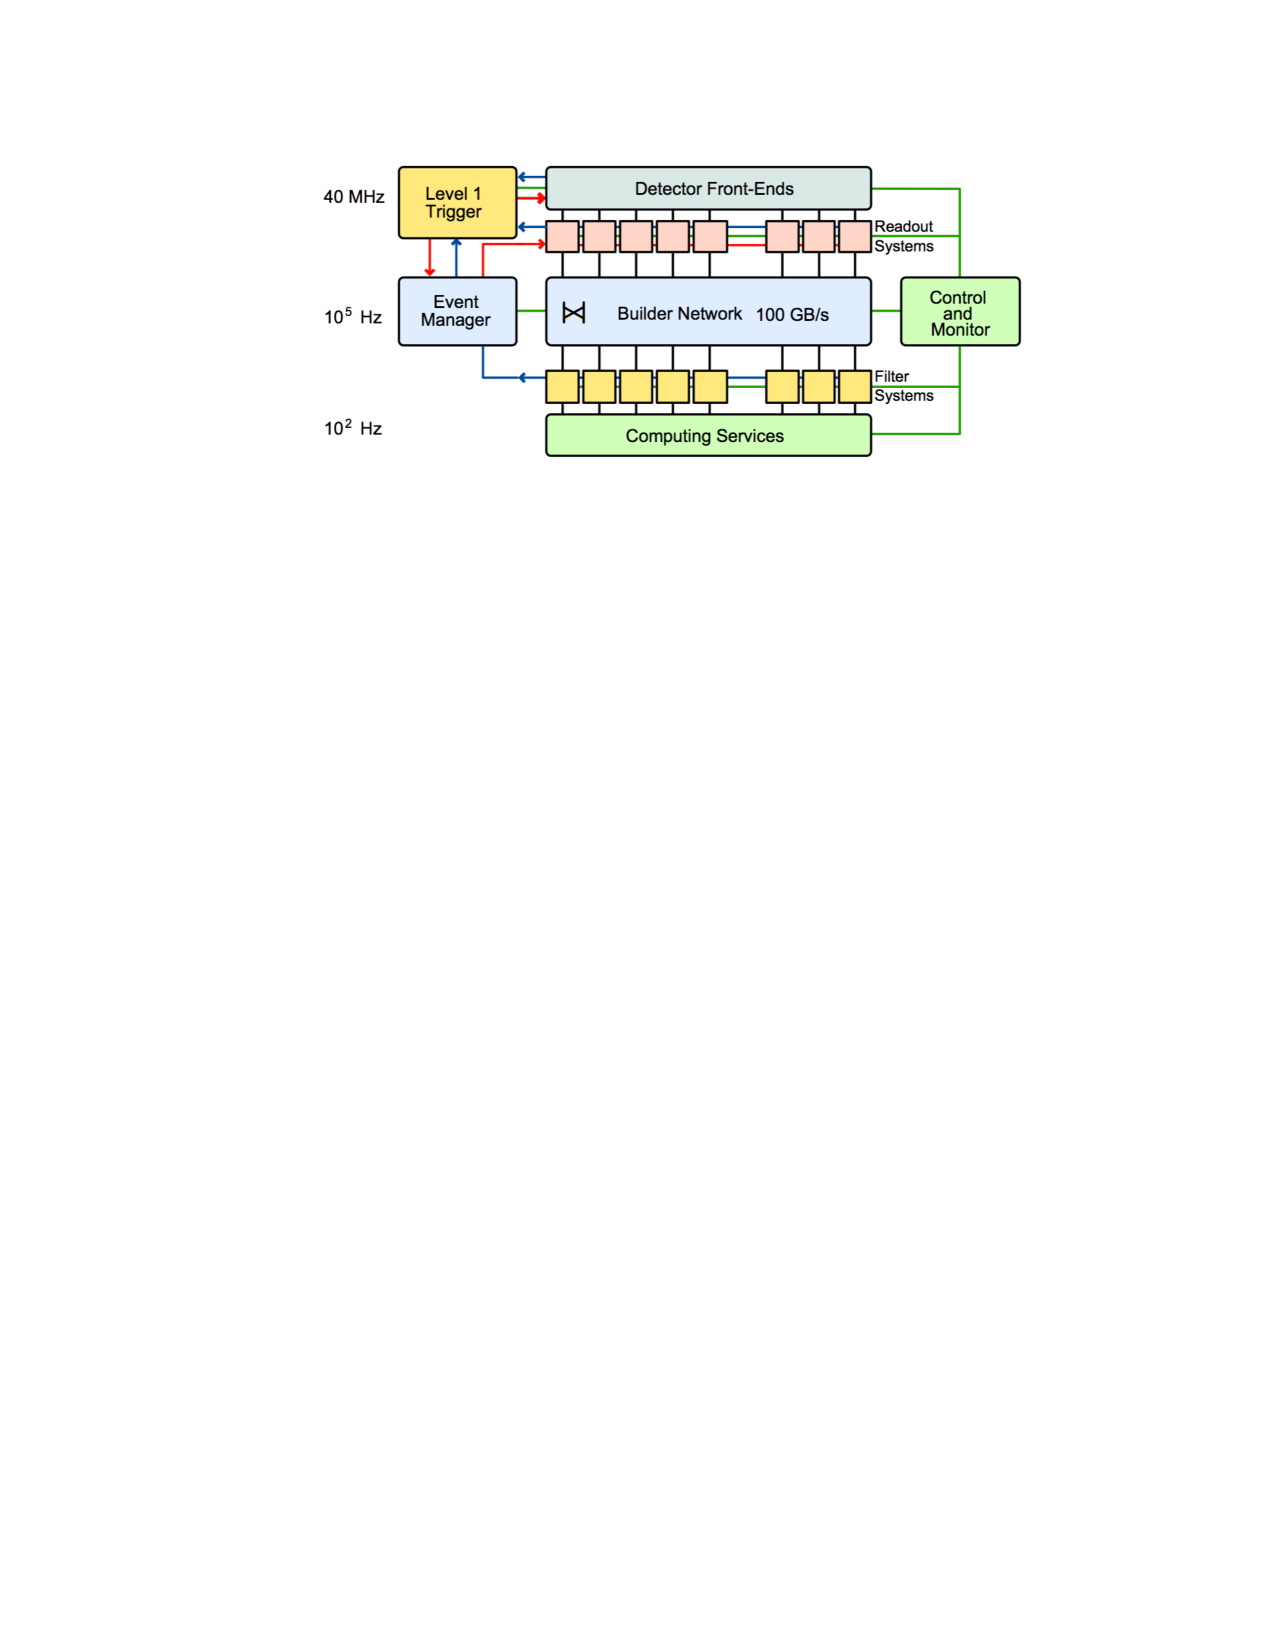
\includegraphics[width=.95\textwidth]{pics/daq_diagram}\\
\caption{A diagrammatic representation of the level 1 and HLT trigger processing}
\label{tab:daq_diagram}
\end{center}
\end{figure}
